\documentclass[type=bachelor]{thuthesis}
% 选项:
%   type=[bachelor], % 必选
%   secret,                                   % 可选
%   pifootnote,                               % 可选(建议打开)
%   openany|openright,                        % 可选,基本不用
%   arial,                                    % 可选,基本不用
%   arialtoc,                                 % 可选,基本不用
%   arialtitle                                % 可选,基本不用

% 所有其它可能用到的包都统一放到这里了,可以根据自己的实际添加或者删除。
\usepackage{thuthesis}

% 定义所有的图片文件在 figures 子目录下
\graphicspath{{figures/}}

% 可以在这里修改配置文件中的定义。导言区可以使用中文。
% \def\myname{薛瑞尼}


\usepackage{listings}
\usepackage{color}
\usepackage{rotating}
\usepackage{makecell}

\definecolor{dkgreen}{rgb}{0,0.6,0}
\definecolor{gray}{rgb}{0.5,0.5,0.5}
\definecolor{mauve}{rgb}{0.58,0,0.82}

\lstset{frame=tb,
  language=Java,
  aboveskip=3mm,
  belowskip=3mm,
  showstringspaces=false,
  columns=flexible,
  basicstyle={\small\ttfamily},
  numbers=none,
  numberstyle=\tiny\color{gray},
  keywordstyle=\color{blue},
  commentstyle=\color{dkgreen},
  stringstyle=\color{mauve},
  breaklines=true,
  breakatwhitespace=true,
  tabsize=3
}

\setcounter{tocdepth}{1}

\begin{document}

%%% 封面部分
\frontmatter
\thusetup{
  %******************************
  % 注意:
  %   1. 配置里面不要出现空行
  %   2. 不需要的配置信息可以删除
  %******************************
  %
  %=====
  % 秘级
  %=====
  secretlevel={秘密},
  secretyear={10},
  %
  %=========
  % 中文信息
  %=========
  ctitle={大规模供电网络分析中线性方程组求解的并行加速算法},
  cdegree={},
  cdepartment={计算机科学与技术系},
  cmajor={计算机科学与技术},
  cauthor={龙浩民},
  csupervisor={蔡懿慈教授},
  % 日期自动使用当前时间,若需指定按如下方式修改:
  % cdate={超新星纪元},
  %
  % 博士后专有部分
  cfirstdiscipline={计算机科学与技术},
  cseconddiscipline={系统结构},
  postdoctordate={2009年7月——2011年7月},
  id={编号}, % 可以留空: id={},
  udc={UDC}, % 可以留空
  catalognumber={分类号}, % 可以留空
  %
  %=========
  % 英文信息
  %=========
  etitle={An Introduction to \LaTeX{} Thesis Template of Tsinghua University v\version},
  % 这块比较复杂,需要分情况讨论:
  % 1. 学术型硕士
  %    edegree:必须为Master of Arts或Master of Science(注意大小写)
  %             “哲学、文学、历史学、法学、教育学、艺术学门类,公共管理学科
  %              填写Master of Arts,其它填写Master of Science”
  %    emajor:“获得一级学科授权的学科填写一级学科名称,其它填写二级学科名称”
  % 2. 专业型硕士
  %    edegree:“填写专业学位英文名称全称”
  %    emajor:“工程硕士填写工程领域,其它专业学位不填写此项”
  % 3. 学术型博士
  %    edegree:Doctor of Philosophy(注意大小写)
  %    emajor:“获得一级学科授权的学科填写一级学科名称,其它填写二级学科名称”
  % 4. 专业型博士
  %    edegree:“填写专业学位英文名称全称”
  %    emajor:不填写此项
  edegree={Doctor of Engineering},
  emajor={Computer Science and Technology},
  eauthor={Xue Ruini},
  esupervisor={Professor Zheng Weimin},
  eassosupervisor={Chen Wenguang},
  % 日期自动生成,若需指定按如下方式修改:
  % edate={December, 2005}
  %
  % 关键词用“英文逗号”分割
  ckeywords={VLSI,供电网络,线性方程组,并行化算法,多重网格},
  ekeywords={VLSI, Power Grid, Linear System, Parallel Algorithm, Multigrid Preconditioner}
}

% 定义中英文摘要和关键字
\begin{cabstract}


  随着大规模集成电路的飞速发展,其供电网络的规模与日俱增,它的计算成本也越来越高。供电网络的仿真设计作为电路设计中最重要的一环之一,影响着电路设计的成败。
  因此供电网络的仿真设计对计算机的计算效率有着非常高的要求。而供电网络的仿真本质上是一个线性方程组的求解问题,解决的方法主要有直接求解法和迭代求解法,都依赖于
  大规模的矩阵、向量运算。

  本文针对供电网络仿真数据的特点,运用了并行计算的技术,对主流的共轭梯度迭代法进行了改进,包括以下创新点:(1)把稀疏矩阵和向量的内容分发到
  计算集群里的不同节点,从而提高了矩阵与向量运算的并行度;(2)针对系数矩阵规模大的特点,选用了多重网格预条件子,使得预条件的计算效率更高。
  我们最后用C++语言与开源的并行计算库在多机集群上实现了一个高效的供电网络仿真算法,并进行了多项测试,证明了算法的有效性。

\end{cabstract}


\begin{eabstract}
   With the fast development of Very Large Scale Integrated circuit, the size of power grid of circuit has increased significantly and become
   more and more computationally challenging both in runtime and memory consumption. The design and simulation of power grid is vital to
   that of the integrated circuit since the former is the most basic and important step of the latter. So the design of power grid is in
   enormouse demand for computational efficiency and ability of the computers. While to solve this problem is to solve a system of linear
   equations, there are two ways to work it out, one is direct method and the other one is iterative method, both of which rely heavily on
   massive matrix and vector operations.

   In this paper, we refine the mainstream iterative method, Conjugate Gradient method by adopting parallel computing techniques and taking
   advantages of the mathematical features of the data in power grid. Our contributions are: (1) Dispatching consecutive contents in matrices
   and vectors to different nodes in a computing cluster, so that we boost the efficiency of matrices and vectors operations by parallel
   computing, (2) Adopting Multigrid preconditioner, which both largely improves the convergence of the linear system and requires relatively
   small amount of computation efforts, based on the fact that the matrix has very sparse coefficients. We implemented an effective algorithm
   with C++ language and with open source parallel computing library on a multi-node cluster. Our experiments on IBM benchmark proved our
   insight in the paper.
\end{eabstract}

% 如果使用授权说明扫描页,将可选参数中指定为扫描得到的 PDF 文件名,例如:
\makecover[scan-auth.pdf]
%\makecover

%% 目录
\tableofcontents

%% 符号对照表
% \begin{denotation}[3cm]
\item[HPC] 高性能计算 (High Performance Computing)
\item[cluster] 集群
\item[Itanium] 安腾
\item[SMP] 对称多处理
\item[API] 应用程序编程接口
\item[PI] 聚酰亚胺
\item[MPI] 聚酰亚胺模型化合物,N-苯基邻苯酰亚胺
\item[PBI] 聚苯并咪唑
\item[MPBI] 聚苯并咪唑模型化合物,N-苯基苯并咪唑
\item[PY] 聚吡咙
\item[PMDA-BDA]	均苯四酸二酐与联苯四胺合成的聚吡咙薄膜
\item[$\Delta G$] 活化自由能 (Activation Free Energy)
\item[$\chi$] 传输系数 (Transmission Coefficient)
\item[$E$] 能量
\item[$m$] 质量
\item[$c$] 光速
\item[$P$] 概率
\item[$T$] 时间
\item[$v$] 速度
\item[劝学] 君子曰:学不可以已。青,取之于蓝,而青于蓝;冰,水为之,而寒于水。木
  直中绳。輮以为轮,其曲中规。虽有槁暴,不复挺者,輮使之然也。故木受绳则直,金就
  砺则利,君子博学而日参省乎己,则知明而行无过矣。吾尝终日而思矣,不如须臾之所学
  也;吾尝跂而望矣,不如登高之博见也。登高而招,臂非加长也,而见者远;顺风而呼,
  声非加疾也,而闻者彰。假舆马者,非利足也,而致千里;假舟楫者,非能水也,而绝江
  河,君子生非异也,善假于物也。积土成山,风雨兴焉;积水成渊,蛟龙生焉;积善成德,
  而神明自得,圣心备焉。故不积跬步,无以至千里;不积小流,无以成江海。骐骥一跃,
  不能十步;驽马十驾,功在不舍。锲而舍之,朽木不折;锲而不舍,金石可镂。蚓无爪牙
  之利,筋骨之强,上食埃土,下饮黄泉,用心一也。蟹六跪而二螯,非蛇鳝之穴无可寄托
  者,用心躁也。—— 荀况
\end{denotation}



%%% 正文部分
\mainmatter
\chapter{引言}
\label{cha:intro}

\section{大规模集成电路与EDA}

集成电路的产生与发展对人类的社会与工业有着重大而深远的影响。下至电脑、手机、相机和各种数字电器,上至人造卫星、火车探测仪,
各种高科技都离不开集成电路的出现。从科学计算到互联网行业,从交通系统到制造业系统,没有一个行业可以脱离集成电路的帮助;
可以说,集成电路已经成为人类社会结构不可或缺的一环了。因此,集成电路的成熟
将会带来科技的大跃进,而科技的进步也会进一步带动集成电路技术的发展;不论是在设计的技术上,或是半导体的工艺突破,两者都是息息相关的。

而自从进入大规模集成电路的时代,集成电路一直遵从这摩尔定律的惊人速度而发展着,其中的晶体管数量,
每1.5年增加一倍。近年来,随着制造工艺与材料工艺的持续发展,芯片的规模增速不见放缓。英伟达公司最新
发布的Tesla V100计算卡,在其815平方毫米的面积上,共有210亿颗晶体管,以及5120个CUDA。这张“巨无霸”
计算卡的出现只是集成电路飞速发展的一个缩影。

早期集成电路规模不大,设计复杂度也不高,设计人员甚至可以手工完成集成电路的设计和优化。到了70年代中期,
集成电路的规模不断增加,程序的仿真模拟与逻辑认证开始被引入到集成电路的开发设计中。为此诞生的电子设计自动化
(Electronic Design Automation,EDA)行业也逐步发展。电子设计自动化不仅减少了人工设计带来的差错,而且
大大提高了电路设计的正确性和容错率。然而随着集成电路的发展,EDA领域也迎来了众多挑战:工艺制造技术发展到32纳米
以下所带来的物理效应、增长迅猛的功耗散热问题、信号完整性问题等~\cite{shang2004thermal, swaminathan2010designing}。

\section{集成电路供电网络的分析与设计}

\begin{figure}[H] % use float package if you want it here
  \centering
  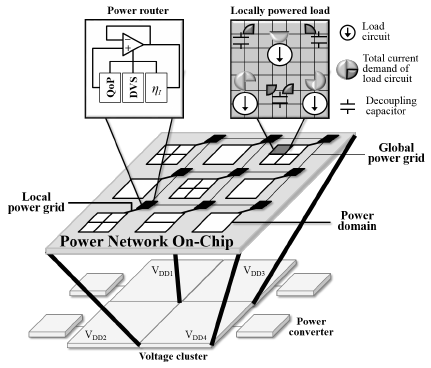
\includegraphics[height=8cm]{power-network-on-chip}
  \caption{集成电路的供电网络}
  \subcaption*{\emph{图片来源:供电网格维基百科}}
  \label{fig:figpower}
\end{figure}

在EDA所关注的问题中,集成电路供电网络的设计~\cite{zhu2004power}是比较重要的一个。通过正确的布线,
可以使得外部电源能给芯片上的各个工作单元提供所需的工作电流,以便正常地工作。由于供电网络涉及到电源线网和
地线网这些关键网络,所以它在布线阶段有着比较高的优先级。对于供电网络来说,它经常使用几层乃至十几层的金属进行
供电线网的设计,占用芯片上的相当一部分资源。

\begin{figure}[H] % use float package if you want it here
  \centering
  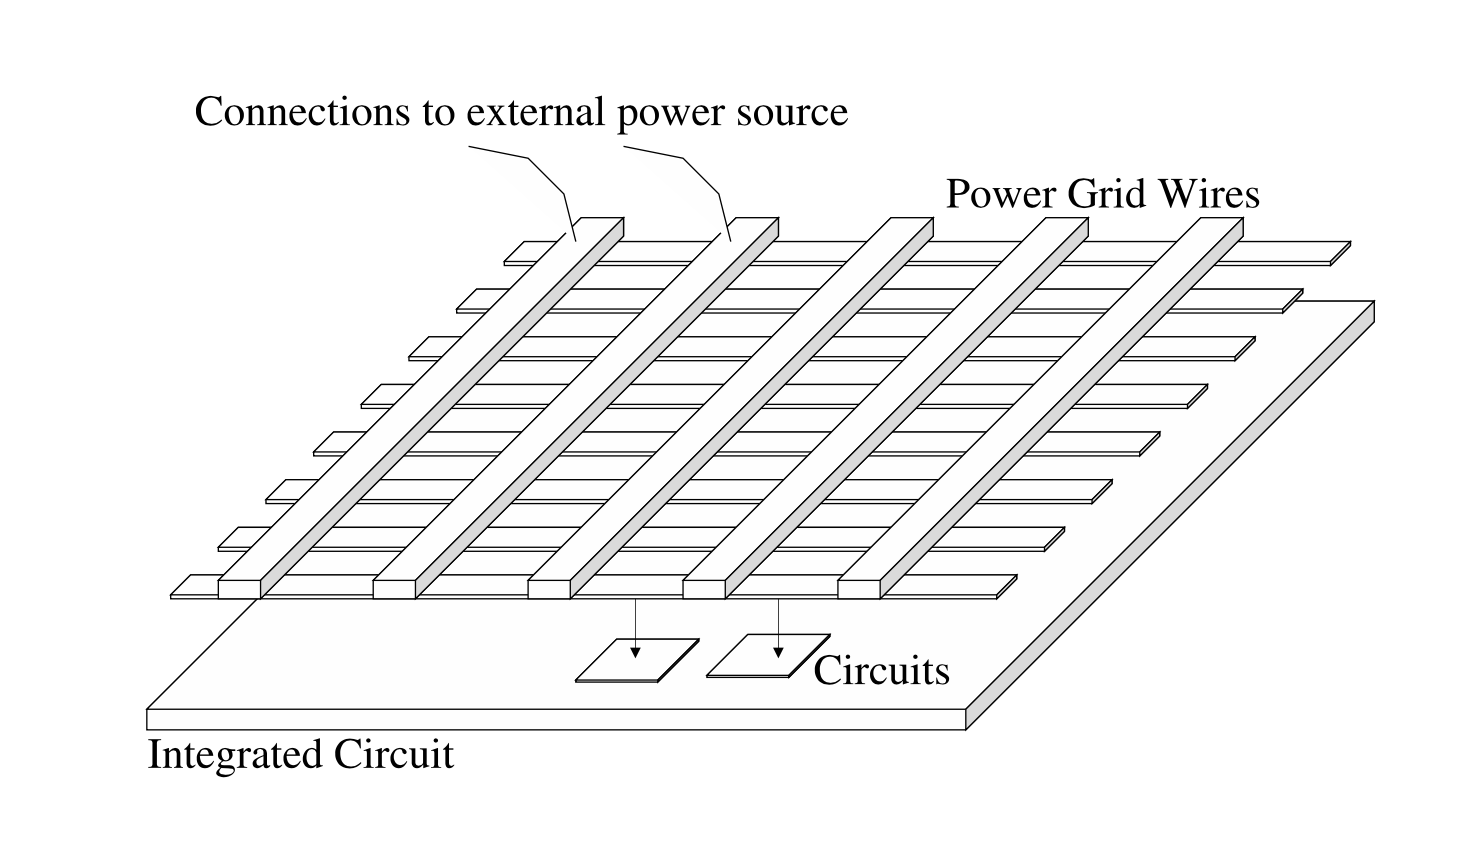
\includegraphics[height=7cm]{power-grid-topology}
  \caption{集成电路的供电网络}
  \subcaption*{\emph{图片来源:供电网格维基百科}}
  \label{fig:figtopology}
\end{figure}

目前各种芯片最常用的供电网络基础结构是一个多层的金属的网格状拓扑图~\cite{popovich2007power}。如图\ref{fig:figpower}与图\ref{fig:figtopology}所示。
对供电网络进行静态仿真分析的时候,可以把这个供电网络当做一个纯电阻网络模型,因此可以采用经典的节点分析法~\cite{vlach1983computer}。节点分析方法中,我们通过建立
并求解一个大规模的线性方程组而得到所有电路网络节点的电压值。对供电网络的进行瞬态仿真分析的时候,情况类似。只需要把储能元件的电容和电感进行离散化,使其等效成为一个常数电阻
并联一个电流源即可。而电流源的值由上一个瞬态计算而得。瞬态仿真通过求解每个时间节点上的电路网络方程,可以得出每个时间节点上的每个电路节点的电压响应,从而为仿真提供电路的动态
变化情况。


\section{供电网络设计遇到的挑战}

同样的,随着集成电路的复杂程度日益增长,供电网络的设计也愈加复杂。这主要是因为~\cite{zhu2004power}:
\begin{enumerate}
    \item 芯片制造工艺尺寸不断降低,集成度越来越高,也就是说芯片的功率密度也越来越高,导致了越来越大的开关电流流经供电网络;
    \item 芯片的晶体管数目增多,功率却要控制住,导致供电电压的阈值一定要控制下来;
    \item 由于供电电压的降低,导致晶体管对噪声的容忍度不断下降,也就对供电网络的设计精度提出了更高的要求;
    \item 随着供电网络晶体管密度的上升,金属走线也越来越窄,带来了不能忽视的寄生电阻、寄生电容效应。
\end{enumerate}

如果从一个更实际的角度去考虑这个问题,可以参考下面两种情况:

\begin{itemize}
\item 在设计一个高性能处理核心的时候,分配10%左右的布线资源到供电网络是很常见的一件事情。这么大的布线资源投入是必须的,因为对于处理器来说,经常用1伏特的电压去
产生100瓦特以上的功耗。所以一旦有1毫欧姆的阻抗,那么就会产生100毫伏特的电压降,也就是电压供应的10\%;这是不可接受的,会降低6\%的处理核心频率,浪费18\%的能源分配;
\item 假设处理核心的结构是八层金属网,占据了一个1cm$\times$1cm的面积,并且使用的线宽是$1\mu$。这意味着每一层金属网格有1000条线路。我们进一步假设线网之间的连接
(via)是纯电阻,那么每一层金属网格会有$10^6$个节点。最后整个处理器核心的供电网络就会有大约$8\cdot 10^6$个节点以及$2.4\cdot 10^7$个电阻;可以说是相当复杂的问题;
\end{itemize}

这些因素导致传统的求解方法越来越不能满足现在的设计需求。如果不能很好地上述这些问题,芯片工艺和材料工艺的进步将被供电网络的设计而限制着。此外,随着
设计越来越复杂,设计周期越来越短,所以早期的供电网络规划愈发重要。如果早期供电网络设计是合理的,并有足够的设计余量,那么即使后期设计中出现供电噪声违规的
现象,也可以通过局部小幅度修改而完成设计需求。相反,如果供电网络的早起设计不合理,那么后期再发现问题的时候,就要把前面的所有设计都推倒重来。

本文的研究工作就是基于这样的挑战而展开的额,针对供电网络分析遇到的挑战,主要围绕大规模供电网络的高性能仿真算法开展深入的研究。

\section{供电网络分析基础}

在介绍本论文的算法之前,先对电路分析的数学背景进行基本的介绍。电路系统一般用三大定律进行描述,包括欧姆定律、基尔霍夫电压定律、基尔霍夫电流定律,通过求解其
一阶非线性差分方程来获得电路各节点、支路的响应。但对于规模较大的实际问题,直接列出方程并求解的效率太低。目前主要使用的电路方程构造方案有:

\begin{itemize}
 \item 稀疏表格方法(Sparse Tableau Analysis,STA)~\cite{hachtel1971sparse}由Hachtel等人于1971年提出。此方法构造出来的电路方程包含所有分支电流、
 分支电压以及节点电压的变量。此方法的适用性非常强,系数矩阵非常稀疏,但是要求解的变量较多。
 \item 改进节点分析方法(Modified Nodal Analysis,MNA)~\cite{ho1975modified}由Ho等人于1975年提出。与STA不同的是,MNA所构造的电路方程组只包含电路节点的
 电压变量以及部分支路电流变量,所以所需求解的变量与方程的规模较STA更小。这是目前最常用的方法。
 \end{itemize}

 \begin{figure}[H]
   \centering
   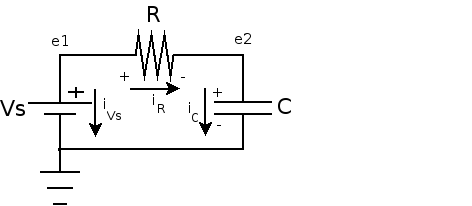
\includegraphics[height=5cm]{simple-circuit}
   \caption{一个简单电路}
   \label{fig:figsimplecircuit}
 \end{figure}

 如图\ref{fig:figsimplecircuit}所示一个简单的电路。如果用电导值$G=\frac{1}{R}$代替电阻值,使用MNA方法可以根据基尔霍夫电压定律列出如下的矩阵方程:

\begin{align*}
 & x=\begin{pmatrix}e_1 & e_2 & i_{V_S}\end{pmatrix}^T, \quad  f=\begin{pmatrix}0 & 0 & V_s \end{pmatrix}^T \\
 \\
 & E=\begin{pmatrix}0&0&0\\ 0&C&0\\ 0&0&0 \end{pmatrix}, \quad A=\begin{pmatrix}G&-G&1\\ -G&G&0\\ 1&0&0 \end{pmatrix}
  \end{align*}

 那么我们可以列出如下的方程:

 \begin{align} E \cdot x'(t) +
  A \cdot x(t) = f \end{align}

 对上列方程进行求解,便可得所求的支路电流值与节点电压值。

 \begin{figure}[H]
   \centering
   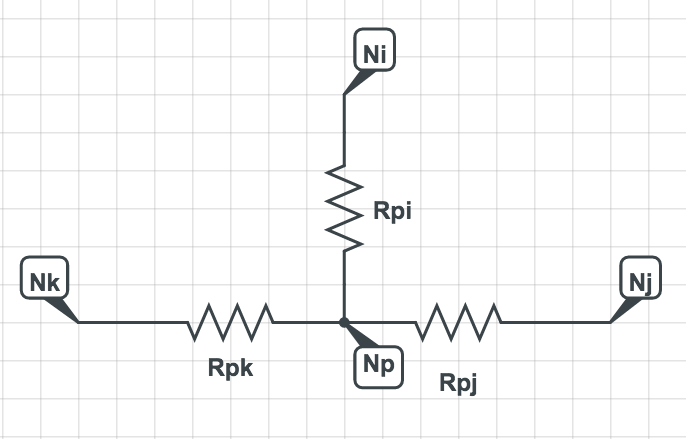
\includegraphics[height=5cm]{mna-demo}
   \caption{改进节点分析方法的系数示意图}
   \label{fig:figmna}
 \end{figure}

 更一般地来说,对于图\ref{fig:figmna}里的一个节点$N_i$来说,它在系数矩阵$A$中对应的元素应该有:

\begin{align}
 \begin{pmatrix}
 & & (i) &  & (j) & & (p) & & (k)& \\
 & & & & & & \vdots & & & \\
 (i) & & & & & & -G_{pi} & & & \\
 & & & & & & \vdots & & & \\
 (j) & & & & & & -G_{pj} & & & \\
 & & & & & & \vdots & & & \\
 (p) & \cdots & -G_{pi} & \cdots & -G_{pj} & \cdots & \sum_{q=\{i,j,k\}} G_{pq}  & \cdots & -G_{pk} & \cdots \\
 & & & & & & \vdots & & & \\
 (k) & & & & & & -G_{pk}& & & \\
 & & & & & & \vdots & & &
 \end{pmatrix}
 \label{Geq}
 \end{align}

也就是说,对于节点$N_p$来说,系数矩阵的第$p$行第$p$列的元素应该是与$N_p$相连的所有电导的和;而其余元素则是对应电导值的相反数。根据这个规则,可以自动化地构造出
电路网络对应的电导矩阵,从而求解电路。

\section{主要工作}

本文的主要工作是根据现有的共轭梯度算法,提出了一种在多机上进行并行计算的加速,并使用多重网格预条件子进行收敛性能的优化。
本文的组成如下:\textbf{第二章}介绍供电网络仿真的相关工作,以及线性方程组求解并行化的研究现状;\textbf{第三章}
介绍了一种基于多重网格预条件子的共轭梯度迭代算法,并提出一种使其在多机上并行计算的方法;
\textbf{第四章}介绍了实验的数据与实验的结果;\textbf{第五章}总结本次毕业设计的工作,回顾不足并展望未来可以继续研究的方向。

\chapter{相关工作与研究现状}
\label{cha:relatedworks}

\section{供电网络的分析与仿真}

大规模供电网络的仿真是一个很成熟的问题。主流的算法可以分成两类:直接求解法和迭代求解法。直接求解法首先通过对矩阵进行分解,然后进行若干次回带便得到解向量;典型的方法有
KLU~\cite{davis2010algorithm}以及Cholmod~\cite{davis2005cholmod}等。
直接求解法通常更加鲁棒,而且求出来的逆矩阵还可以复用;但所需要的内存过多,随着问题规模的扩大而急剧增长,不能处理越来越大的供电网络。
迭代求解法通常先设定一个初始解,然后构造具有一定性质的迭代序列,如果问题满足一定的条件的话最终会收敛到方程的解。迭代求解法所需要的计算资源更少,尤其是遇到大规模的电路矩阵时;
然而迭代求解法的计算不够稳定,对于有病态性的问题收敛速度非常慢。2001年,Chen等人提出用预条件子的Krylov子空间迭代法~\cite{chen2001efficient},
这个方法比当时传统的直接求解方法要快了10倍左右,并且有更好的收敛性质。之后,各种预条件子都被提出来,包括随机行走~\cite{qian2005power},
多重网格方法~\cite{kozhaya2002multigrid},层次方法~\cite{zhao2002hierarchical}等。


\section{线性方程组的求解}

在高性能计算的领域,线性方程组的并行加速是一个被广泛研究但仍然十分活跃的问题。Saad的著作~\cite{saad2003iterative}中有对这个问题涉及到的并行数值计算以及各类
迭代算法有入门的介绍,里面介绍了:稀疏矩阵的矩阵向量乘法操作(Sparse Matrix-Vector Multiplication,SPVM),基于Jacobo或者SSOR预条件子的Krylov子空间方法等内容。
Lee等人的论文~\cite{lee2004performance}深入介绍了计算密集的SPVM操作的各种研究和优化。作者在论文里提出了一种对算法参数进行调节的方法,这个方法基于经验模型和一定程度的
搜索算法。

共轭梯度算法~\cite{hestenes1952methods}(Conjugate Gradient Method,CG)由Hestenes等人提出,在数值计算领域有着非常悠久而成功的应用历史。
Van der Sluis等人研究了CG算法的收敛性能~\cite{van1986rate}及其Ritz值的关系。

在描述网格型的拓扑结果,或者计算偏微分方程的离散化形式的时候,经常会出现规模巨大、系数十分稀疏的矩阵,因此SPVM操作在该类数值计算中十分重要。而当矩阵与向量的数据分布在
不同计算节点的时候,SPMV操作会带来巨大的通讯开销。所以在对数据进行节点分发的的时候,通常会选择一种分发方式,使得跨节点的数据访问尽可能地少出现。
Demmel等人的报告~\cite{demmel1993parallel}中提出了一些能够同时进行数据传输与数值计算(也就是两种操作并行进行)的预条件共轭梯度算法(Preconditioned Conjugate Gradient Method, PCG),从而使得在一定程度上掩盖通讯时间过长的问题。

近年来,越来越多研究开始尝试使用图形处理核心(Graphics Processing Unit,GPU)来解决非图形相关的问题,加速计算密集的任务。Owens等人的报告~\cite{owens2007survey}
介绍了这些趋势。

\chapter{并行化加速的预条件共轭梯度算法}
\label{cha:algo}

\section{供电网络的抽象数学模型}

由于本数据集是瞬态的直流DC网络,所以网络中只有三种基本元件:电阻、独立电压源、独立电流源。为了建立改进节点分析方法的方程,先根据
电路里的连接关系建立系数矩阵$A$:对于连接节点$i$与节点$j$的支路$k$,如果这个支路的方向是从$i$到$j$,那么$A_{k,i}=1, A_{k,j}=-1$;
如果支路的方向是从$j$到$i$,那么$A_{k,i}=-1, A_{k,j}=1$;其余情况$A$的元素为0。

更进一步的,根据支路$b$是纯电阻支路、电压源支路、电流源支路可以把$A$按列分成三部分$A_G,A_V,A_I$。同样的对于支路电流向量$i$,可以分成$i_G,i_V,i_I$;
对于节点电压向量$v_b$,可以分成$v_G,v_V,v_I$。
\begin{align}
A=\begin{bmatrix} A_I \\ A_V \\ A_G \end{bmatrix}, \quad
i_b=\begin{bmatrix} i_I \\ i_V \\ i_G \end{bmatrix},\quad
v_b=\begin{bmatrix} v_I \\ v_V \\ v_G \end{bmatrix}
\end{align}
那么根据基尔霍夫电压定律和基尔霍夫电流定律可以写出($v_n$是节点电压向量):
\begin{align}
A^T i_b & =  0 \\
A v_n & = v_b
\end{align}
展开上述两个式子可得:
\begin{align*}
A_I^T i_I + A_V^T i_V + A_G^T i_G & = 0 \\
A_I v_n & = v_I \\
A_V v_n & = v_V \\
A_G v_G & = v_G \\
i_I & = I \\
v_V & = V \\
i_G & = P v_G \\
\end{align*}
其中$P$是电导邻接矩阵:如果支路$k$上存在阻值为$R$、连接$i$到$j$的电阻,那么$P_{k,i}=\frac{1}{R}$,$P_{k,j}=\frac{1}{R}$。

根据改进节点分析方法的原理,可以通过简化去掉所有支路电压的变量,也就是$v_b$;以及大部分支路电流变量,也就是$i_b$。
化简后可以得到:
\begin{align}
    A_G^T P A_G v_n + A_V^T i_V & = -A_I^T I    \\
    A_V v_n & =V
\end{align}
令$G=A_G^T P A_G$,其中$G$也就是在公式\ref{Geq}中提到的电导矩阵。那么可以得到:
\begin{align}
    \begin{bmatrix}
    G & A_V^T \\
    A_V & 0 \\
    \end{bmatrix}
    \begin{bmatrix}
    v_n \\ i_V
    \end{bmatrix}
    =
    \begin{bmatrix}
    0 & -A_I^T  \\
    1 & 0
    \end{bmatrix}
    \begin{bmatrix}
    V \\ I
    \end{bmatrix}
    \label{eqbasic}
\end{align}

式\ref{eqbasic}的右边是确定的,左边有一个未知向量$x=\begin{bmatrix}v_n \\ i_V\end{bmatrix}$,因此可以使用线性方程求解器进行求解。此外,系数矩阵
可以看出来非常稀疏并且是对角占优的,因此有很多优化的余地。但是,值得注意的是系数矩阵并不是对称正定的,所以像Cholesky Solver这种算法就不能再用了。

\subsection{处理节点间的短路}

由于系数矩阵使用的是电导值,所以节点间的短路并不能直接用阻值为0的电阻代替。为了解决这个问题,考虑对于一个电路来说,由短路的节点组成的集合等效于一个超节点,也就是说
我们可以把它们当做一个节点来处理。实现的时候,对于短路的节点集合,我们新建一个超节点表示它们的等效节点,与这个超节点相连的所有支路是这些短路的节点的支路的并集,这个
超节点挂载的电流源负载是这些短路的节点的电流源负载之和。

此外,为了求出超节点,在处理读入数据的时候,我们采用了并查集~\cite{tarjan1975efficiency}的方法,即维护一个图的森林,一开始所有节点都是森林里的孤立的节点;如果读入两个节点$i$和$j$是短路的,那么找到节点$i$所在的连通块的根节点,把这个根节点挂在节点$j$下,也就是成为$j$的子节点;最后所有节点的关系形成了一个森林,森林里每个连通块都是
一个超节点。

\section{解线性方程的共轭梯度算法}

求解式\ref{eqbasic}中的线性方程组有两种基本方法:直接求解法与间接迭代法。直接求解法的算法鲁棒性更强,但是由于该线性方程组的节点规模非常巨大,直接求解法会要求
过多的CPU计算资源与内存,无法解决问题。迭代法由于预条件子的问题,求解稳定性不如直接求解法,但是更加节省计算资源,是解决该问题的合适方法。对于本问题,我们采取经典的基于预条件子的共轭梯度法(Preconditioned Conjugate Gradient Method,PCG)进行求解。下文探讨的主要是对此算法的优化。

没有用预条件子的共轭梯度算法如下所示:
\begin{lstlisting}
//算法1.cpp
r[0] = b - A * x0;
p[0] = r[0];
k = 0;
repeat
    alpha[k] = dot(r[k], r[k]) / dot(p[k], A * p[k]);
    x[k+1] = x[k] + alpha[k] * p[k];
    r[k+1] = r[k] - alpha[k] * A * p[k];
    if r[k+1]足够小
        break;
    else
        beta[k] = dot(r[k+1], r[k+1]) / dot(r[k], r[k]);
        p[k+1] = r[k+1] + beta[k] * p[k];
        k = k + 1;
    end if
end until
求解结果为x[k+1]
\end{lstlisting}

但是共轭梯度算法的求解速度,也就是收敛速度取决于系数矩阵$A$的条件数。为了改善这一点,我们可以用一个预条件子$M$对系数矩阵$A$进行预处理,使得$M^{-1}A$的条件数尽量小。
使用预条件子后的算法如下:
\begin{lstlisting}
//算法2.cpp
r[0] = b - A * x0;
z[0] = inverse(M) * r[0]
p[0] = z[0];
k = 0;
repeat
    alpha[k] = dot(r[k], z[k]) / dot(p[k], A * p[k]);
    x[k+1] = x[k] + alpha[k] * p[k];
    r[k+1] = r[k] - alpha[k] * A * p[k];
    if r[k+1]足够小
        break;
    else
        z[k+1] = inverse(M) * r[k+1];
        beta[k] = dot(z[k+1], z[k+1]) / dot(z[k], z[k]);
        p[k+1] = z[k+1] + beta[k] * p[k];
        k = k + 1;
    end if
end until
求解结果为x[k+1]
\end{lstlisting}

\section{预条件子??}

\section{多机并行优化中的线程级优化}

实现算法的时候,我们在两个方面进行了并行优化:线程级和进程级的优化。实验时使用具有八个核心(CPU Processor)的机器,我们在每个核心上使用八个线程并行进行各种矩阵运算,包括
向量内积、矩阵与向量的乘法、向量加法等,从而最大程度地发掘算法的并行性。

首先,为了进行线程级的优化,我们直接使用了OpenMP代码库提供的API。OpenMP(Open Multi-Processing)是一套支持跨平台共享内存方式的多线程并发的编程API,使用C/C++和Fortran语言,可以在大多数的处理器体系和操作系统中运行具体的实现。OpenMP提供了对并行算法的高层的抽象描述,程序员通过在源代码中加入专用的pragma来指明自己的意图,由此编译器可以自动将程序进行并行化,并在必要之处加入同步互斥以及通信。当选择忽略这些pragma,或者编译器不支持OpenMP时,程序又可退化为通常的程序(一般为串行),程序码仍然可以正常运作,只是不能利用多线程来加速程序执行。一个典型的例子如下:
\begin{lstlisting}
//dot_product.cpp
int ComputeDotProduct(const int n, const Vector & x, const Vector & y, double & result) {
  result = 0.0;
  double * xv = x.values;
  double * yv = y.values;
  #pragma omp parallel for reduction (+:result)
  for (local_int_t i=0; i<n; i++)
    result += xv[i]*yv[i];
  return 0;
}
\end{lstlisting}

上述例子中,通过pragma指令,我们实现了向量内积算法中的线程级并行化。实现的方法是在可以并行执行的循环代码前加pragma指令,这样编译器就会自动生成相应的代码,在循环代码前
派生出若干个线程,不同线程之间并行执行,执行完后汇集到父线程上。
需要注意的是,由于不同线程的计算累加结果是分开存储的,所以要在pragma指令中指明对result变量进行reduction操作,从而把所有线程计算的结果累加存储在result变量中。
使用OpenMP之前,要注意判断代码中是否有数据依赖的部分;如果有,要尽量去掉,保证代码的可并行性。

\section{多机并行优化中的进程级优化}

虽然上一小节中提到的线程级的优化对程序效率已经有了不少提升,但是还远远不够。因为线程级的并行化要求共享内存,也就是所有数据都存储在本机上;此外,单机的
处理能力是有限的,本实验的数据规模较大,需要更多的计算资源。为此,需要进行多机的并行化处理,也就是进程级的并行优化。进程级的并行加速能最大程度地同时发掘多台机器的
计算能力,非常适合解决这种大规模的计算问题。但是与线程级的优化不同,进程与进程之间的内存是不共享的,因此进程与进程之间需要相互通信,从而同步计算的数据。对于进程级
的并行化来说,通信带来的时间与空间开销往往限制了算法的优劣程度以及算法的并行化程度。通常来说,进程、机器越多,通讯的花销越大,性能有可能不如使用进程更少的算法。
\begin{figure}[H]
  \centering
  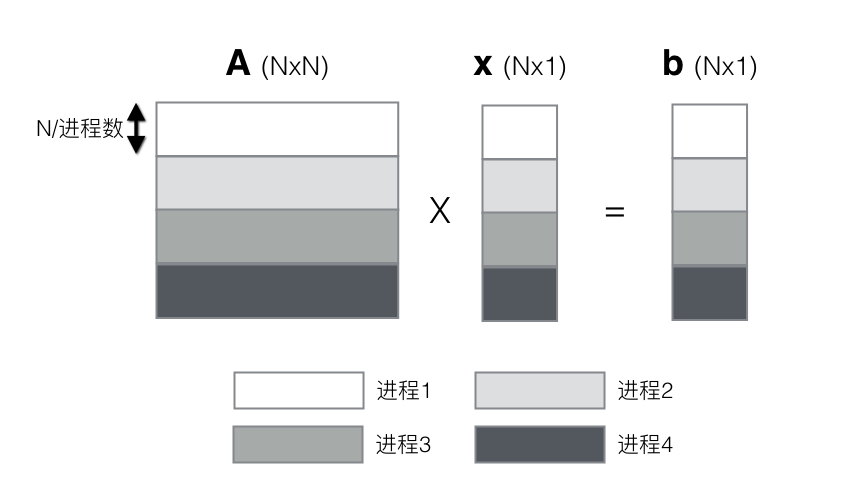
\includegraphics[height=8cm]{paral_demon}
  \caption{MPI中的负载平衡}
  \label{fig:figparaldemon}
\end{figure}

对于本实验来说,我们需要把进程的并行化运用到共轭梯度算法中。注意到系数矩阵非常稀疏,并且具有局部性。
那么一种可行的办法是把矩阵中连续的行分配给每一个进程,如图\ref{fig:figparaldemon}所示:若系数矩阵的
大小为$N\times N$,共有$K$个进程,那么第一个进程计算$x_1,\ldots,x_{\frac{N}{k}}$,第二个进程计算计算$x_{\frac{N}{k}+1},\ldots,x_{2\frac{N}{k}}$,
依次类推。也就是对于进程$i$来说,他只负责计算和保存$x_{(i-1)\frac{N}{k}+1},\ldots,x_{i\frac{N}{k}}$的值。所以在第$i$个进程迭代更新$x$的值的时候,需要
通过通讯手段来获得其余$x$(不在这个进程上)的值。在程序中,由于这一点,我们不能再用变量x来访问整个向量,因为内存中只存有该向量的部分内容(下文中用
local\_x来表示本地进程中的x的值)。为了正确地执行原算法,我们必须在进程中进行必要的通讯以交换不同进程的内容。

对于共轭梯度算法来说,主要的数学运算与对应的通讯方法如下:

\begin{itemize}
\item 计算向量$x$和$y$的内积。由于本进程中只有local\_x与local\_y的内容,所以每个进程先计算各自local\_x与local\_y的内积,存为local\_result,即本地结果;然后
把各自的本地结果广播给其他进程,从而完成本地结果的累加,计算出全局的内积;
\item 计算向量$x$和$y$的和。直接计算即可,不需要通讯,因为向量加法对于各个元素来说是独立的;
\item 计算矩阵$A$和向量$x$的乘积$y$。因为计算结果$y$是局部的,也就是只需要计算$y_{(i-1)\frac{N}{k}+1},\ldots,y_{i\frac{N}{k}}$,所以只需存储系数矩阵A的第
$((i-1)\frac{N}{k}+1)$到$(i\frac{N}{k})$行;此外,如果存在非零系数$A_{i,j}$,那么计算结果时就需要$x_j$的值;所以我们需要预处理出每一个$y_i$所需要的非局部的
$x$值,并通过通讯手段从其他进程中获取其值。
\end{itemize}

改动后的算法3如下:
\begin{lstlisting}
//算法3.cpp
local_r[0] = local_b - local_A * local_x0;
syncGlobal(sync_r, local_r);
local_z[0] = inverse(M) * sync_r[0];
local_p[0] = local_z[0];
k = 0;
repeat
    //get global dot(r,z)
    local_rtz = dot(local_r[k], local_z[k]);
    getGlobal(global_rtz, local_rtz);
    //get global dot(p,Ap)
    syncGlobal(sync_p, local_p);
    local_Ap = local_A * sync_p;
    local_pAp = dot(local_p[k], local_Ap);
    getGlobal(global_pAp, local_pAp);
    //compute alpha
    alpha[k] = global_rtz / global_pAp;
    //compute x
    local_x[k+1] = local_x[k] + alpha[k] * local_p[k];
    local_r[k+1] = local_r[k] - alpha[k] * local_Ap[k];
    if r[k+1]足够小
        break;
    else
        syncGlobal(sync_r, local_r)
        local_z[k+1] = inverse(M) * sync_r[k+1];
        beta[k] = global_rtz / old_rtz;
        old_rtz = global_rtz;
        local_p[k+1] = local_z[k+1] + beta[k] * local_p[k];
        k = k + 1;
    end if
end until
求解结果为x[k+1]
\end{lstlisting}
其中,主要的通讯函数有:
\begin{enumerate}
    \item getGlobal(global\_data, local\_data)函数,作用是通过通讯手段从其他进程中获取、接受它们各自的local\_data值,并统计到global\_data变量中(合并结果的
    方法有累加、取最大值、取最小值等);
    \item syncGlobal(result, local\_data)函数,作用是通过通讯手段,从其他进程中获取、接受local\_data对应的变量的部分全局值,并存在result变量中;
\end{enumerate}

与单机上的原算法相比,使用了多进程并行化优化的算法3在矩阵运算方面处理的数据规模更小,比如所处理的向量长度从原来的$N$降到了$N/\text{处理器数量}$,因此减少了程序的
数学运算量;并且,利用矩阵与向量运算的各元素独立性,不同的进程之间可以并行执行各种运算,因此大大提高了程序运行的时间利用率;但是算法引入了另外一种开销:通讯开销。比如
在计算向量内积时,需要等待所有进程都计算完本地局部内积后再相加,才可以得出总体的内积;在计算矩阵与向量的乘积时,需要从其它进程中接收某些非本地向量元素,也需要把本地的
向量元素发送到其它有需要的进程里。可以看出,进程数越多,算法的并行度越高,计算本地结果的效率越高,但是花在通讯上的花销会更大;进程数越少,算法并行度越低,但是通讯代价
会降低。

在本实验中,多机的并行通讯采用了消息传递接口(Message Passing Interface,MPI)的标准。MPI是一个跨语言的通讯协议,用于编写并行计算机。支
持点对点和广播。MPI是一个信息传递应用程序接口,包括协议和和语义说明,他们指明其如何在各种实现中发挥其特性。

\section{本章小结}

本章介绍了供电网络的抽象数学模型的建立,以及解决其相应的线性方程组的方法。基于现有的共轭梯度算法,作者实现了多机多核并行的算法,并进一步分析了这个算法的性能。最后,为了提高算法的性能,作者又引入了基于多重网格的预条件子,从而解决了问题病态下的收敛速度的问题。

\chapter{新算法的实验结果}
\label{cha:exp}

\section{IBM的测试数据集}

这一小节讲介绍测试数据集中关于供电网络的模型假设。此数据集来源于IBM的公开数据~\cite{nassif2008power}。

此数据集共有六个电路参考设计,分别命名为IBMPG1到IBMPG6。表格\ref{tab:tabibm}总结了这几个设计的重要特征参数,包括电路的节点数、包含的纯电阻个数、包含的电压源与电流源个数、
金属层数等。整个数据集的节点数量之间的差距在两个数量级之间。

\begin{table}[htbp]
\centering
\caption{IBM供电网络测试集合}
\label{tab:tabibm}
\begin{tabular}{|c|r|r|r|r|r|r|}
\toprule[1.5pt]
\hline
数据编号 & 电流源数量 & 节点数量 & 电阻数量 & 短路数量 & 电压源数量 & 金属层数 \\
\hline
IBMPG1 & 10774 & 30638  & 30027  & 14208  &  14308 & 2\\
\hline
IBMPG2 & 37926 & 127238 & 208325 & 1298  & 330 & 5\\
\hline
IBMPG3 & 201054 & 851583 & 1401572 & 461 & 955 &  5\\
\hline
IBMPG4 & 276976 & 953583 & 1560645 & 11682 & 962  & 6\\
\hline
IBMPG5 & 540800 & 1079310 & 1076848 & 606587 & 539087 &  3\\
\hline
IBMPG6 & 761484 & 1670494 & 1649002 & 836107 & 936239 &  3\\
\hline
\end{tabular}
\end{table}

数据集文件用SPICE格式存储。具体的格式说明如下:

\begin{itemize}
\item 如果一行以星号(*)开头,那么这一行是注释;
\item 每一层电路的数据开头有一行注释:\emph{layer: <层名>,<网层> net: <网层序号>},例如\emph{layer: M1,Vdd net: 1}与\emph{layer: M1,Vss net: 2};
\item 层与层之间的连接(vias)数据前面会有一行注释:\emph{vias from: <网层序号> to <网层序号>};
\item 电路的节点形式为:\emph{n<网格序号>\_<节点x坐标>\_<节点y坐标>},例如"n3\_124\_921";
\item 如果一行的第一个字母是R,那么这一行的格式形如"Rxxxx Node1 Node2 value",其中“xxxx”是该电阻的名字(没有实际作用。可以忽略),表示Node1与Node2之间
有一个阻值为value的电阻;
\item 如果一行的第一个字母是V,那么这一行的格式形如"Vxxxx Node1 Node2 value",其中“xxxx”是该vias的名字(没有实际作用。可以忽略),表示Node1与Node2之间
有一个阻值为value的vias;value的值可以为0,表示这两个节点被短路了(通常用在两层之间相同位置的节点上);
\item 如果一行的第一个字母是r,那么这一行的格式形如"rxxxx Node1 Node2 value",其中“xxxx”是该电阻的名字(没有实际作用。可以忽略),表示Node1与Node2之间
有一个阻值为value的电阻;小写字母r开头的电阻与大写字母R的电阻的不同之处在于,小写字母r表示的是节点Node1和某个package(也就是Node2)(?)之间的电阻;例如Node1
如果名字是"n3\_123\_456",那么Node2一定是"\_X\_n3\_123\_456",所以这一行的形式为"rxxxx n3\_123\_456 \_X\_n3\_123\_456"。特殊的,电路数据文件里会指定这个package
的电压值,形式为"vxxxx Node2 0 value"其中Node2为小写字母r开头的数据中指定的package,value为该Node2的电压值;
\item 最后,负载电流源的形式为"iBxxxx Node 0 value"或者"iBxxxx 0 Node value“;分别表示从节点到Vdd的电流源大小或者从Vss到节点的电流大小。
\end{itemize}

\begin{figure}[H]
  \centering
  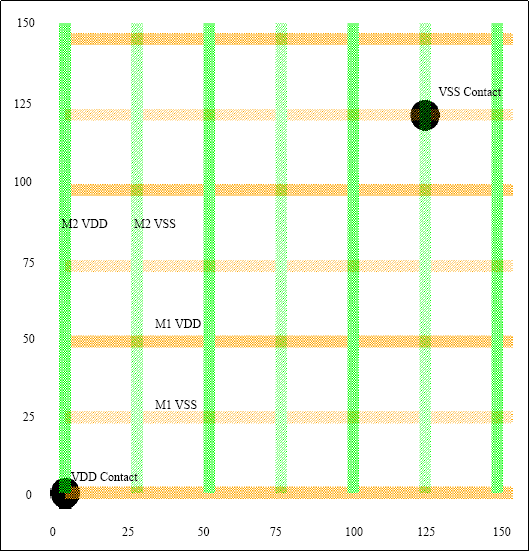
\includegraphics[height=8cm]{sample1}
  \caption{IBM供电网络测试数据集的数据样例}
  \label{fig:figsample1}
\end{figure}

图\ref{fig:figsample1}是一个比较小的供电网络例子。这个例子总共有两层金属网格,分别是水平排列的M1和垂直排列的M2;每一层金属网格都有4个Vdd线路和3个Vss线路;此供电网络
有两个package(用黑色实心圆圈表示),一个接电源,另一个接地。

它的数据如下:

\begin{lstlisting}
rr0 n3_0_0 _X_n3_0_0 0.5
v1 _X_n3_0_0 0 1
rr2 n2_125_125 _X_n2_125_125 0.5
v3 _X_n2_125_125 0 0
* layer: M1,VDD net: 1
R4 n1_0_0 n1_50_0 1.25
R5 n1_50_0 n1_100_0 1.25
R6 n1_100_0 n1_150_0 1.25
R7 n1_0_50 n1_50_50 1.25
R8 n1_50_50 n1_100_50 1.25
R9 n1_100_50 n1_150_50 1.25
R10 n1_0_100 n1_50_100 1.25
R11 n1_50_100 n1_100_100 1.25
R12 n1_100_100 n1_150_100 1.25
R13 n1_0_150 n1_50_150 1.25
R14 n1_50_150 n1_100_150 1.25
R15 n1_100_150 n1_150_150 1.25
* vias from: 1 to 3
V16 n1_0_0 n3_0_0 0.0
V17 n1_0_50 n3_0_50 0.0
V18 n1_0_100 n3_0_100 0.0
V19 n1_0_150 n3_0_150 0.0
V20 n1_50_0 n3_50_0 0.0
V21 n1_50_50 n3_50_50 0.0
V22 n1_50_100 n3_50_100 0.0
V23 n1_50_150 n3_50_150 0.0
V24 n1_100_0 n3_100_0 0.0
V25 n1_100_50 n3_100_50 0.0
V26 n1_100_100 n3_100_100 0.0
V27 n1_100_150 n3_100_150 0.0
V28 n1_150_0 n3_150_0 0.0
V29 n1_150_50 n3_150_50 0.0
V30 n1_150_100 n3_150_100 0.0
V31 n1_150_150 n3_150_150 0.0
* layer: M2,VDD net: 3
R32 n3_0_0 n3_0_50 1.25
R33 n3_0_50 n3_0_100 1.25
R34 n3_0_100 n3_0_150 1.25
R35 n3_50_0 n3_50_50 1.25
R36 n3_50_50 n3_50_100 1.25
R37 n3_50_100 n3_50_150 1.25
R38 n3_100_0 n3_100_50 1.25
R39 n3_100_50 n3_100_100 1.25
R40 n3_100_100 n3_100_150 1.25
R41 n3_150_0 n3_150_50 1.25
R42 n3_150_50 n3_150_100 1.25
R43 n3_150_100 n3_150_150 1.25
* layer: M1,GND net: 0
R44 n0_25_25 n0_75_25 1.25
R45 n0_75_25 n0_125_25 1.25
R46 n0_25_75 n0_75_75 1.25
R47 n0_75_75 n0_125_75 1.25
R48 n0_25_125 n0_75_125 1.25
R49 n0_75_125 n0_125_125 1.25
* layer: M2,GND net: 2
R50 n2_25_25 n2_25_75 1.25
R51 n2_25_75 n2_25_125 1.25
R52 n2_75_25 n2_75_75 1.25
R53 n2_75_75 n2_75_125 1.25
R54 n2_125_25 n2_125_75 1.25
R55 n2_125_75 n2_125_125 1.25
* vias from: 0 to 2
V56 n0_25_25 n2_25_25 0.0
V57 n0_25_75 n2_25_75 0.0
V58 n0_25_125 n2_25_125 0.0
V59 n0_75_25 n2_75_25 0.0
V60 n0_75_75 n2_75_75 0.0
V61 n0_75_125 n2_75_125 0.0
V62 n0_125_25 n2_125_25 0.0
V63 n0_125_75 n2_125_75 0.0
V64 n0_125_125 n2_125_125 0.0
*
iB0_0_v n1_0_0 0 0.3125m
iB0_0_g 0 n0_25_25 0.3125m
iB0_1_v n1_0_50 0 0.3125m
iB0_1_g 0 n0_25_25 0.3125m
iB0_2_v n1_0_100 0 0.3125m
iB0_2_g 0 n0_25_75 0.3125m
iB0_3_v n1_0_150 0 0.3125m
iB0_3_g 0 n0_25_125 0.3125m
iB0_4_v n1_50_0 0 0.3125m
iB0_4_g 0 n0_25_25 0.3125m
iB0_5_v n1_100_0 0 0.3125m
iB0_5_g 0 n0_75_25 0.3125m
iB0_6_v n1_50_50 0 0.3125m
iB0_6_g 0 n0_25_25 0.3125m
iB0_7_v n1_50_100 0 0.3125m
iB0_7_g 0 n0_25_75 0.3125m
iB0_8_v n1_100_50 0 0.3125m
iB0_8_g 0 n0_75_25 0.3125m
iB0_9_v n1_100_100 0 0.3125m
iB0_9_g 0 n0_75_75 0.3125m
iB0_10_v n1_50_150 0 0.3125m
iB0_10_g 0 n0_25_125 0.3125m
iB0_11_v n1_100_150 0 0.3125m
iB0_11_g 0 n0_75_125 0.3125m
iB0_12_v n1_150_0 0 0.3125m
iB0_12_g 0 n0_125_25 0.3125m
iB0_13_v n1_150_50 0 0.3125m
iB0_13_g 0 n0_125_25 0.3125m
iB0_14_v n1_150_100 0 0.3125m
iB0_14_g 0 n0_125_75 0.3125m
iB0_15_v n1_150_150 0 0.3125m
iB0_15_g 0 n0_125_125 0.3125m
\end{lstlisting}

\section{实验平台}

实验使用的集群由8个节点组成,每个节点是一个Xeon E5-2699v4。Xeon E5-2699v4属于Intel Xeon®系列的处理器,有22个核心,基础频率是
2.20GHz,最高可超频至3.60GHz;并有55MB的智慧缓存(Smart Cache),支持DDR4 SDRAM内存。节点之间用Enhanced Data Rate(EDR)的Infiniband连接着,
EDR的传输速率可以达到100Gb/s。每一个节点有128GB的内存。

\section{预条件子算法与并行化的实验结果分析}

本文使用C++语言实现第三章中的算法,编译器是Intel CC 17.0.4,MPI库使用的是Intel MPI 2017.3.196。

程序时间的测量使用的是系统时钟,运行时间没有包括数据读入和输出的时间。在正确性校验中,比较的标准是计算出来的电压值不能与标准值(由IBM测试集提供)差距超过$10^{-3}$,
也就是1毫伏。

对于每个测试点,我们分别用1个、2个、4个、8个计算节点(核心)对其进行多进程测试,以此来考察并行化对算法的加速效果。

\begin{sidewaystable}[htbp]
\centering
\caption{IBM数据集的测试结果}
\label{tab:tabibmresult}
\begin{tabular}{c|r|r|r|r|r|r|r|r}
\toprule[1.5pt]
\hline
数据编号 & 节点数量 & \textbf{计算节点数} & 迭代次数 & 通讯总量 & 非零元数量 & \makecell{通讯总量\\/非零元数量} & 运算时间(秒)
& \makecell{ \textbf{加速比} \\ \textbf{(相比单个运算节点)} } \\
\hline
IBMPG1 & 16327  & 1 & 172   &  0 & 75827 & 0\% & 0.427 & 1.000\\
\hline
& & 2 & 238 & 3438 & 75827 & 4.53\% & 0.119 & 3.602 \\
\hline
& & 4 & 254 & 6810 & 75827 &  8.98\% &  0.068 & 6.304 \\
\hline
& & 8 & 261 & 11208 & 75827 & 14.78\% & 0.081 & 5.265 \\
\hline
IBMPG2 & 126905 & 1 & 244 & 0 & 542895 & 0\% & 3.003 & 1.000 \\
\hline
& & 2 & 394 & 163410 & 542895 & 30.01\% & 1.291 & 2.325 \\
\hline
& & 4 & 405 & 172544 & 542895 & 31.78\% &  0.700 & 4.290 \\
\hline
& & 8 & 488 & 185346 & 542895 & 34.13\% & 0.459 & 6.543 \\
\hline
IBMPG3 & 285344 & 1 & 271 & 0 & 1508802 & 0\% & 9.663 & 1.000 \\
\hline
& & 2 & 412 & 18660 & 1508802 & 1.23\% & 5.241 & 1.844 \\
\hline
& & 4 & 471 & 262662 & 1508802 & 17.41\% & 3.600 & 2.685 \\
\hline
& & 8 & 510 & 319344 & 1508802 & 21.17\% & 2.447 & 3.948 \\
\hline
IBMPG4 & 952618 & 1 & 337 & 0 & 4054056 & 0\% & 41.532 & 1.000 \\
\hline
& & 2 & 563 & 1273824 & 4054056 & 31.421\% & 29.840 & 1.392 \\
\hline
& & 4 & 576 & 2136810 & 4054056 & 52.71\% & 19.695 & 2.101 \\
\hline
& & 8 & 568 & 2250576 & 4054056 & 55.51\% & 12.198 & 3.405 \\
\hline
IBMPG5 & 540220 & 1 & 336 & 0 & 2691958 & 0\% & 25.119 & 1.000 \\
\hline
& & 2 & 466 & 116832 & 2691958 & 4.34\% & 13.088 & 1.919 \\
\hline
& & 4 & 528 & 155100 & 2691958 & 5.76\% & 8.757 & 2.869 \\
\hline
& & 8 & 523 & 177632 & 2691958 & 6.60\% & 5.459 & 4.601 \\
\hline
IBMPG6 & 834252 & 1 & 390 & 0 & 4125504 & 0\% & 43.936 & 1.000 \\
\hline
& & 2 & 582 & 11148 & 4125504 & 0.27\% & 26.389 & 1.665 \\
\hline
& & 4 & 571 & 227452 & 4125504 & 5.51\% & 15.453 & 2.843 \\
\hline
& & 8 & 558 & 339142 & 4125504 & 8.22\% & 9.834 & 4.468 \\
\hline
\end{tabular}
\end{sidewaystable}

如果一个并行化算法是理想的,即忽略通讯交换数据带来的开销以及数据依赖带来的阻塞问题,那么算法的执行效率应该随着核心数的增加而线性增加,如图\ref{fig:figspeedupratio}
中的黑色虚线所示(其中,加速比的定义是串行算法的运行时间除以并行算法的运行时间;在本实验中,串行算法就是只有1个计算节点的情况,即单机执行;并行算法就是使用
多个计算节点的情况)。图\ref{fig:figspeedupratio}比较了理想情况下的加速比与实验中的加速比,可以看出,对于每个测试点,随着进程数/核心数的增加,
运行的时间是近线性地减少的。唯一的例外是IBMPG1对应的蓝色曲线,有一个拐点。这是因为IBMPG1的数据规模比较小,程序运行时间较短,所以并行化的效果并不显著。

需要注意的是,在使用不同数量的计算节点的时候,共轭梯度算法的迭代次数变化非常小,因此可以得出:在运算总次数极不不变的情况下,处理运算的运行效率提升了,
也就是说执行各种矩阵向量计算的效率也提升了。这证明了并行化算法的有效性。

此外,根据表格\ref{tab:tabibmresult},随着进程数/核心数的增加,通讯的代价也在增长,这主要体现在计算SPVM与向量内积时的数据通信上。当有多个计算节点时,一个节点
需要从系数矩阵中对应行涉及的列所在的节点中接受那些节点本地保存着的变量值;由于系数矩阵的对称性,这个节点也要发送本地的变量值给那些节点。具体来说,如果系数矩阵$A$的
第$i$行第$j$列不为0,即$A_{i,j}\neq 0$,并且行$i$与行$j$保存在不同的计算节点上时,这两个节点就要互相发送、接受$x_i$与$x_j$。
对于本算法来说,通讯的花销可以通过计算这样的$A_{i,j}$的数量来实现。这样的$A_{i,j}$越多,意味着在单次SPVM运算中节点间的通讯量越大。

图\ref{fig:figcomm}与\ref{fig:figcomm2}中有计算节点数与通讯量的关系图。为了让通讯量在电路节点数不同的数据之间可以比较,可以使用(计算节点数$/$系数矩阵非零元)来表示相对通讯量的大小。
总的来说,通讯的花销阻碍了程序效率的进一步提升,导致算法的加速比没有达到理想的情况。在IBMPG6的测试中,使用了八个计算节点的并行化算法,相比单机算法只有4.468的加速比。



\begin{figure}[H]
  \centering
  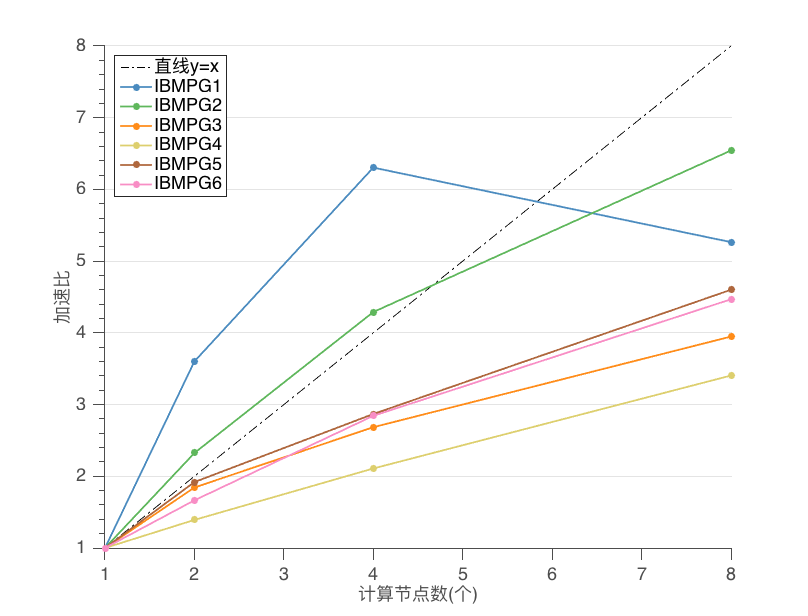
\includegraphics[height=10cm]{speedup-ratio}
  \caption{加速比与计算节点数的关系}
  \label{fig:figspeedupratio}
\end{figure}

\begin{figure}[H]
  \centering
  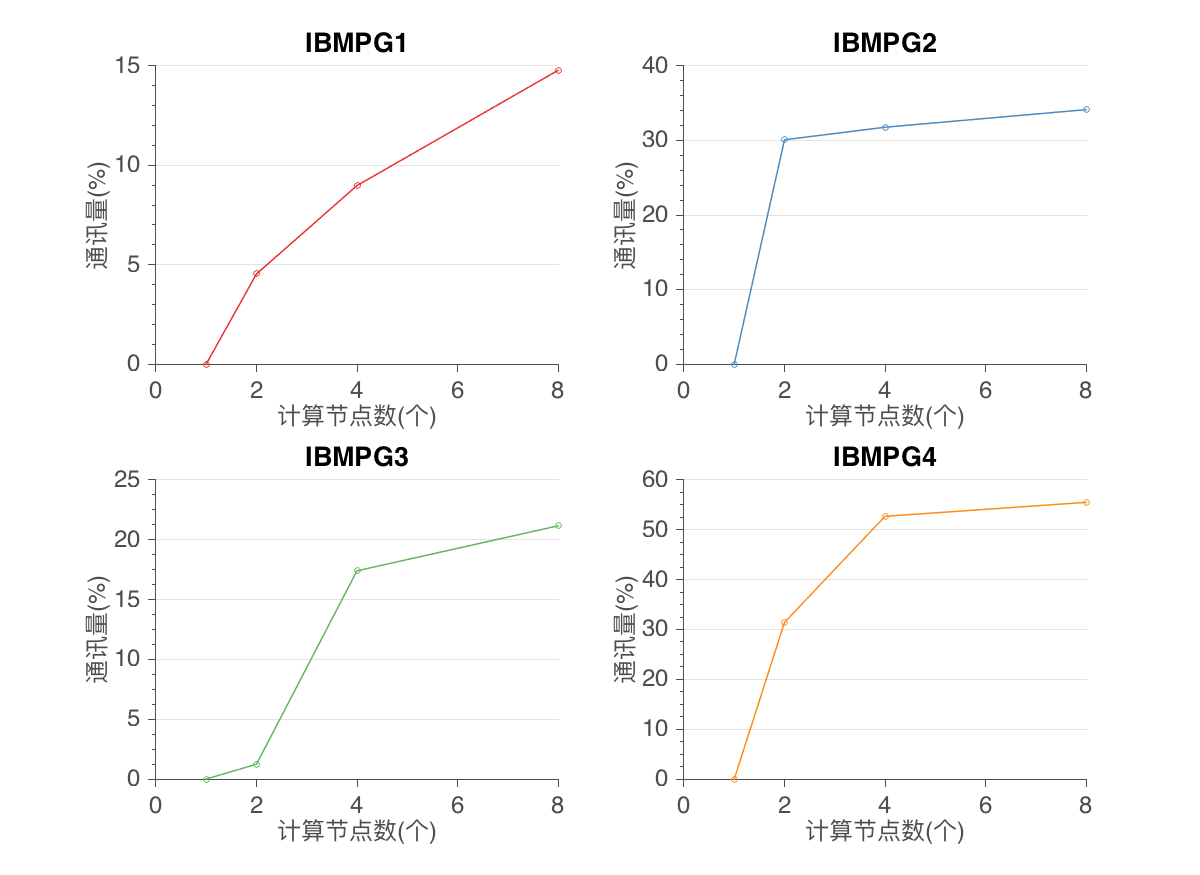
\includegraphics[height=9.6cm]{comm}
  \caption{通讯量与计算节点数的关系}
  \label{fig:figcomm}
\end{figure}


\begin{figure}[H]
  \centering
  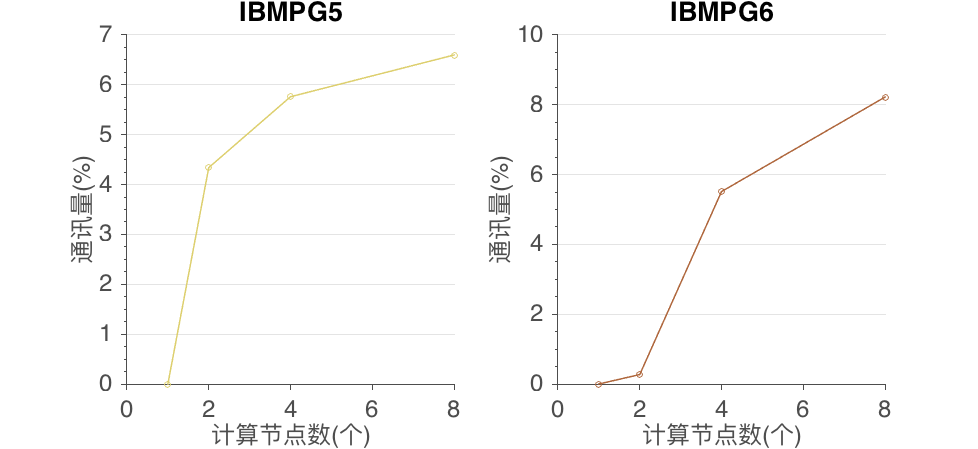
\includegraphics[height=5.7cm]{comm2}
  \caption{通讯量与计算节点数的关系2}
  \label{fig:figcomm2}
\end{figure}

\section{本章小结}

本章通过对IBM的供电网络数据集的实验,证明了第三章中提出的算法的正确性与有效性。其中,并行化对程序的效率提升起到了关键的作用:随着进程数
/使用的核心数的增加,共轭梯度算法中的各种基本运算操作都得到了有效的并行加速,从而使得程序的效率呈近线性增加;虽然在进程间通讯方面有一定的开销,
但效率的提升仍然显著。除了并行化,多重网格预条件子也对算法的效率提高起到很重要的作用,增加了收敛的速度,大大减少了迭代的次数。

\chapter{总结与未来展望}
\label{cha:conclusion}



%%% 其它部分
\backmatter

%% 本科生要这几个索引,研究生不要。选择性留下。
% 插图索引
\listoffigures
% 表格索引
\listoftables
% 公式索引
\listofequations


\bibliographystyle{thuthesis-numerical}
\bibliography{ref/refs}


%% 致谢
% 如果使用声明扫描页,将可选参数指定为扫描后的 PDF 文件名,例如:
\begin{acknowledgement}[scan-statement.pdf]
  衷心感谢导师蔡懿慈教授对本人的精心指导。她的言传身教将使我终生受益,她对我的谆谆教导对我意义重大。

  衷心感谢父母在我成长的路上给予我无私的爱,以及无微不至的关怀;感谢弟弟一直以来陪伴着我。

  感谢301宿舍各位同学在这4年里对我的启发和帮助。感谢王邈同学与李宇轩同学为我提供的计算资源。

  感谢\thuthesis,它的存在让我的论文写作轻松自在了许多,让我的论文格式规整漂亮了许多。
\end{acknowledgement}


%% 附录
\begin{appendix}
\chapter{外文资料翻译}
\label{cha:engorg}

\title{A Multigrid-like Technique for Power Grid Analysis}
\begin{center}\emph{Joseph N. Kozhaya, Sani R. Nassif, and Farid N. Najm}\end{center}
\textbf{摘要}:
现代的超大规模集成电路设计里面包括规模巨大的供电网络,供电网络需要用越来越低的电压分配大量的供电源。网格中的电压降减少了噪声区间的范围,增加了门延迟,造成了一系列的
性能影响。用传统的电路模拟方法对供电电压的完整性进行检验是一个不现实的方法,因为时间与内存开销过大。我们提出了一个新的基于多重网格的供电网络分析技术。原供电网格
被缩小到一个更粗的网格结构,然后这个网格的解会被映射回原来的细网格中。实验结果证明了我们提出的方法效率非常高,适合供电网格的直流分析与瞬态分析。

\section{引言}

近年来,对高性能与低能耗的VLSI设计的需求越来越高。高性能的实现主要通过技术扩大,功能增强以及更好的设计。另一方面,一个常用的低能耗的设计方法是减少供电电压,因为
芯片功率$P$是与供电电压$V_{DD}$的平方成正比的。所以,对于高性能与低能耗的需求导致了现代的VLSI设计以少量的特点大小、增强的功能、低供电电压为特点。

增强的芯片功能导致了对巨大功率分布网络的需求,这也被成为供电网格因为他们经常是一个网格状的拓扑结构。更低的供电电压,另一方面,使得电压在供电网格范围内的抖动会带来
很大的影响,进一步会导致电路的故障。电压值的降低会使得逻辑门与晶体管元件的实际供电电压比理论值要小。这会导致更窄的噪声区间,更高的逻辑门延迟,以及整个电路的降速。
噪声区间变窄会导致电路里特定逻辑门的错误的开关切换。更高的逻辑门延迟在另一方面也会降低电路的速度导致时序要求无法满足。所以,一旦电压的降低超过了一定的设计阈值,
电路的正常运行就没法保证了[1],[2],[3]。

因此,很显然在现代的VLSI设计中,供电网格正在成为制约性能的一个重要因子。所以对供电网格的高效分析[4][5]是很有必要的;
一能预测性能,二能改善性能。因为供电网格的规模大的特性,现在的分析方法都不能满足需求。所以,一个时间与内存效率都高的分析技术显得格外重要。

\section{供电网格的建模与分析}

在这一节中,我们会讨论供电网格的基本模型与分析技术。具体来说,第二节节会讨论如何对传统的供电网格、电流源、二极管进行建模,以适应高效精确的分析。另一方面第三节会
介绍基本的分析技术并讨论一些提升分析速度的技术细节。

\subsection{供电网格的建模}


从供电网格到外部供能电源($V_{DD}$)的连接被称为电力来源,因为电流是通过这个连接从外部电源流入网格的。电源漏极,另一方面,指的是那些从供电网格中获取电流的元件。比如说,
晶体管、逻辑门、触发器、时钟缓存器、内存单元、寄存器阵列、IO缓存区等都被认为是电源漏极。

供电网格分析的第一步包括对电网以及电源和漏极进行建模[6]。 网格,电力来源和漏极的建模涉及准确性和速度之间的权衡。 模型越复杂分析结果越准确,
解决方案越昂贵(在内存和CPU时间方面)。

\begin{figure}[H] % use float package if you want it here
  \centering
  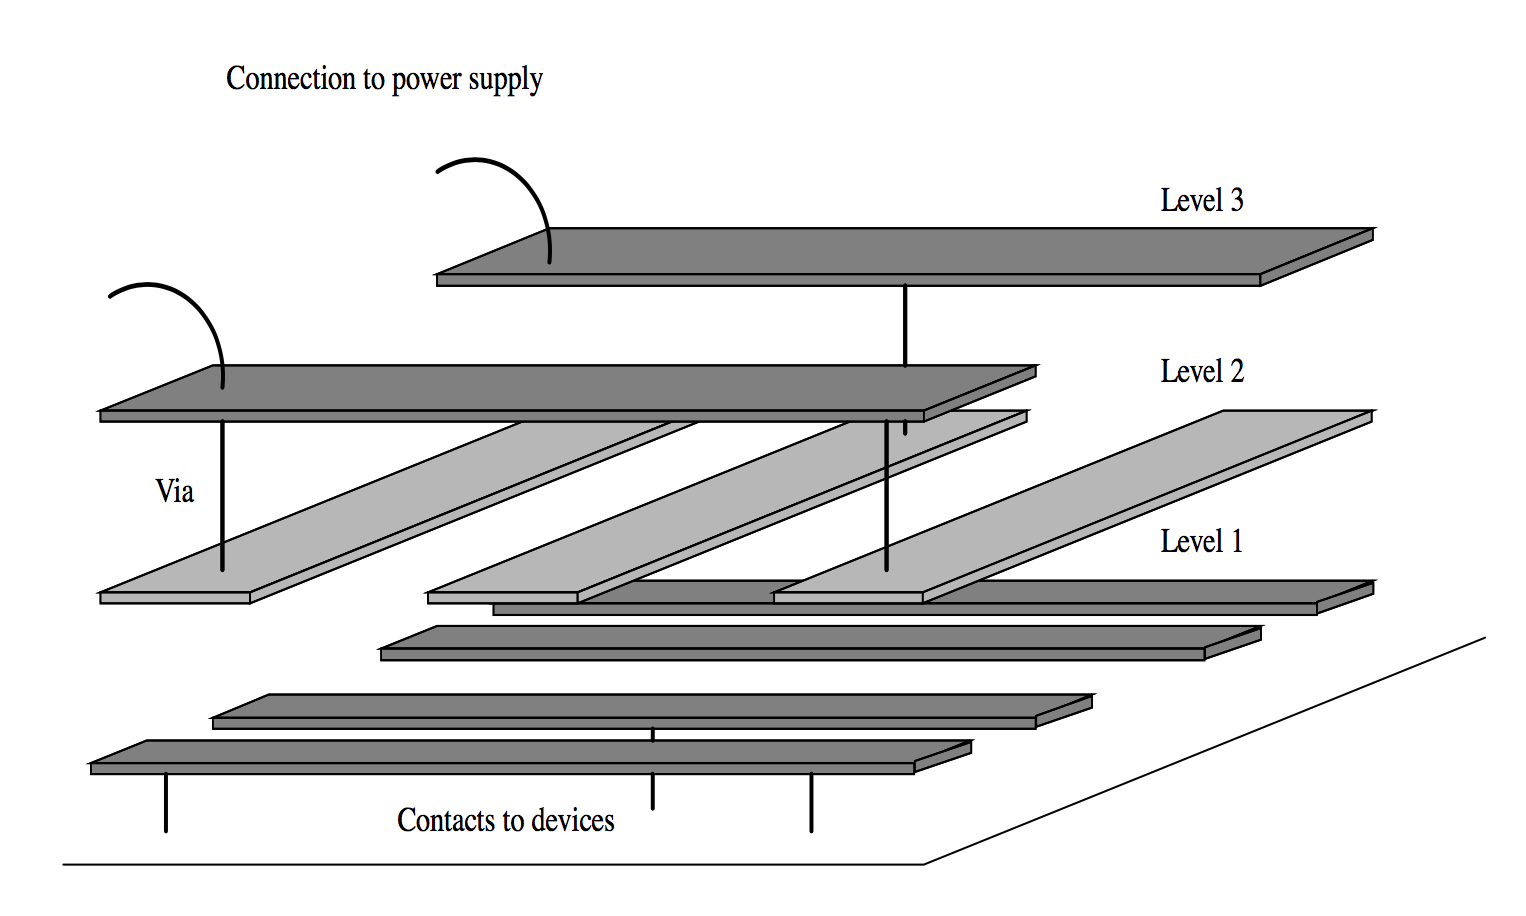
\includegraphics[height=8cm]{a1}
  \caption{供电网络的组成}
  \label{fig:a1}
\end{figure}

通常,如图\ref{fig:a1}所示,集成电路内的功率分配由顶层金属层完成,顶层金属层通过层间通孔向下连接,最后到达目标器件。我们遵循如[6]所述的建模方法,其中金属线和通孔被建模为由电阻性,电容性和非电感性元件组成的线性、时不变的网络。 对于诸如微处理器的现代集成电路,这样的网络可以轻易地包括数百万个节点和数千万个元件。

至于电源和漏极,其型号可能相当复杂。 电源的型号包括复杂的封装和电路板型号。 另一方面,电源漏极的模型可以解释供电网格,底层非线性电路与跨芯片传播的时变信号之间的复杂相互作用。 然而,供电网格巨大的规模使得电源和漏极系统中只能使用最简单的模型。 因此,电力来源被建模为简单的恒定电压源,功率消耗被建模为独立的时变电流源。

鉴于上述情况,完整的供电网格模型由一个由恒定电压源和时变电流源激励的RLC元件组成的线性网络。 需要注意的是,没有任何网络的RLC元件是连接到地的,所有的电压源都在某些网格节点和地之间,并且所有的电流源(漏极)都在网格节点和地之间。 这种系统的行为可以通过修改的节点分析(MNA)[7]公式来表达:
\begin{align}
Gx+C\dot{x}=u(t)
\label{eq:eq1}
\end{align}
其中$x$是节点电压、电源、电导电流的向量;G是电导矩阵;C包括电容和电感项,$u(t)$包括电力来源和漏极的贡献。 事实上,$u(t)$具有三种行:i) 具有正$V_{DD}$值的行,其对应于连接到电源的节点,ii) 具有负电流值(或电流总和)的行,其对应于连接到一个或多于一个功率消耗的节点,以及iii) 具有0的行,其对应于所有其他节点。

接下来,我们忽略片上电感的影响,并假设电网仅被建模为RC网络。 这是由于在当今的技术中,电网中的片上电感太小而不能显著影响分析结果。 总而言之,电网被建模为RC网络,电源被建模为恒定电压源,功率消耗被建模为时变电流源。

\begin{figure}[H] % use float package if you want it here
  \centering
  \includegraphics[height=5cm]{a2}
  \caption{3x3的供电网格例子}
  \label{fig:a2}
\end{figure}

\begin{figure}[H] % use float package if you want it here
  \centering
  \includegraphics[height=3cm]{a3}
  \caption{逆转器引去的电流}
  \label{fig:a3}
\end{figure}

图\ref{fig:a2}表示出了在节点1处具有一个电压源(由X指示)和节点5和7处的两个电流源(由点指示)的$3x3$电网。 该示例表示出在每层中具有三根电线,节点1处有一个电压源,有两个功率消耗(一个从节点5引去电流,另一个从节点7引去电流)的两层电网的模型。一个关联着逆转电源漏极的电流源的示例如图\ref{fig:a3}所示,以数学的形式表达如下(其中$t$是以纳秒为单位的时间,I是以毫安为单位的电流):

\begin{align}
I=\begin{cases}
    410^6t & 0\leq t \leq 0.2510^{-9}\\
    -410^6 + 210^{-3} & 0.2510^{-9} \leq t \leq 0.510^{-9}
\end{cases}
\end{align}

\subsection{供电网格的分析}

由于供电网格的大规模,一般电路仿真器如Spice[8]不足以进行电网分析,因为CPU时间和内存有一定的限制。 标准模拟器的低效率是因为 (a)它们需要电路的元件都近似,该电路需要将常规的电路几何结构转换成一组扩展的等效电路元件,(b)它们使用通用的解决方法, 即使是难解的方程组也要保证正确性。 相比之下,供电网格在空间(非常规则)和时间(阻尼性的)方面表现良好。 这让我们想到了一种可以利用这些特性的供电网格专用模拟器。

求解式子\ref{eq:eq1}需要使用一些数值积分公式。 通常会选择逆向欧拉(BE)积分公式,主要是由于其稳定性的特点[7]。对式子\ref{eq:eq1}应用后向欧拉得到一组线性方程:
\begin{align}
(G+C/h)x(t+h)=u(t+h)+x(t)C/h
\label{eq:eq2}
\end{align}
可以被简化成$A'x(t+h)=b'$,其中$A'=G+C/h$并且$b'=u(t+h)+x(t)C/h$。

式子\ref{eq:eq2}的解决方案要求矩阵$A'= G + C / h$的逆矩阵,其独立于x,时不变,规模大但是系数稀疏。 然而,我们注意到,如果我们将时间步长h保持恒定,那么只需要一个初始的矩阵分解,和每个时间步长的向前/向后的解。 因为对于大规模的矩阵,矩阵分解比前向/后向解决方案明显更花销更高[9],所以使用恒定的时间步长可以大大节省计算成本。 时间步长需要保持足够小以确保解决方案的准确性。 为了在数字电路的电网分析中的应用,我们发现每个时钟周期使用100个步长(即$h = 0.01 * T$)就足够了。

\begin{figure}[H] % use float package if you want it here
  \centering
  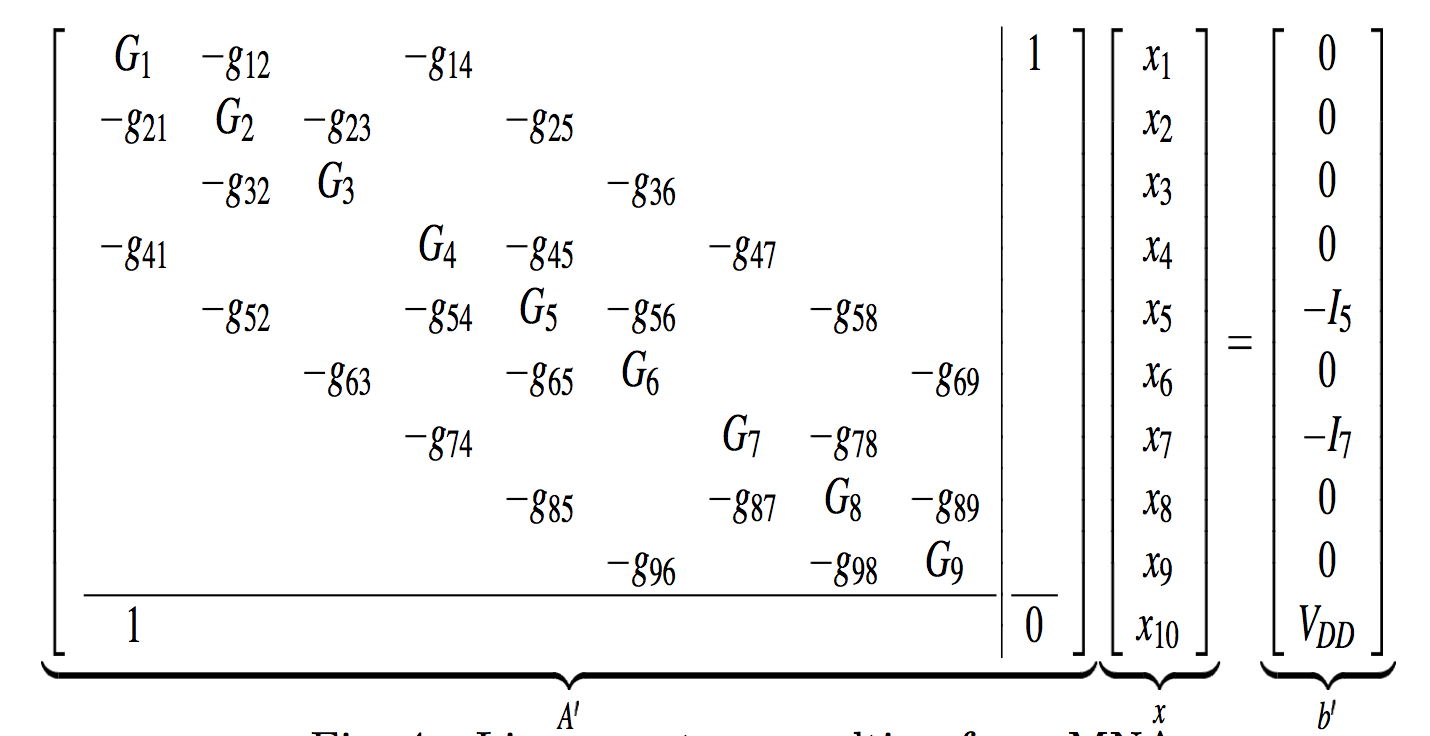
\includegraphics[height=5cm]{a4}
  \caption{根据修改的节点分析法得到的矩阵}
  \label{fig:a4}
\end{figure}

为了更好地解释供电网格的分析过程,将修改的节点分析法(MNA)应用于图\ref{fig:a2}给出的示例,从而得到了图\ref{fig:a4}所示的线性系统。

令$N$为电网的节点数。 然后,在图\ref{fig:a2}所示的示例网格中,$N = 9$,因为网格是3x3。此外,存在一个电压源,这意味着$A'$矩阵是10x10矩阵,其中前9个方程是应用KCL方程在所有9个节点上,最后一个方程是节点1处的电压源分配的KVL方程。 电流源方面,节点5和7中的电流源出现在右侧矢量$b'$中。 另一方面,$g_{ij}$定义了两个相邻节点$i$和$j$之间的电导。 因此,$g_{ij} = g_{ji}$导致$A'$矩阵是对称的。 此外,A矩阵的对角元素定义如下:
\begin{align}
    G_i = \sum_{j\in N_i} |g_{ij}| + C_i/h
    \label{eq:eq3}
\end{align}
其中,$C_i$是节点$i$的电容,$h$是时间步长,$N_i={j|g{ij}\neq 0}$是节点$i$的邻接点集合。

通常,线性系统$A'x = b'$的系统矩阵$A'$是对称的,但不一定是正定的[9]。然而,该问题可以被重新归纳到对称的正定矩阵$A$上。基本上,MNA公式通过在电源节点处运用KCL和KVL方程来构建线性系统$A'x = b'$,以及剩下的网格节点的KCL方程。然后,所得到的线性系统的解$x$给出了所有电网节点处的电压以及由不同电压源提供的电流。然而,如果我们只对所有电网节点的电压感兴趣,那么我们可以忽略与电源节点相对应的KCL方程。此外,电源节点处的电压已知为电源电压$V_{DD}$。因此,我们可以通过将电源的值替换为所有电源节点的电压,并忽略电源节点的KCL方程来简化问题。

\begin{figure}[H] % use float package if you want it here
  \centering
  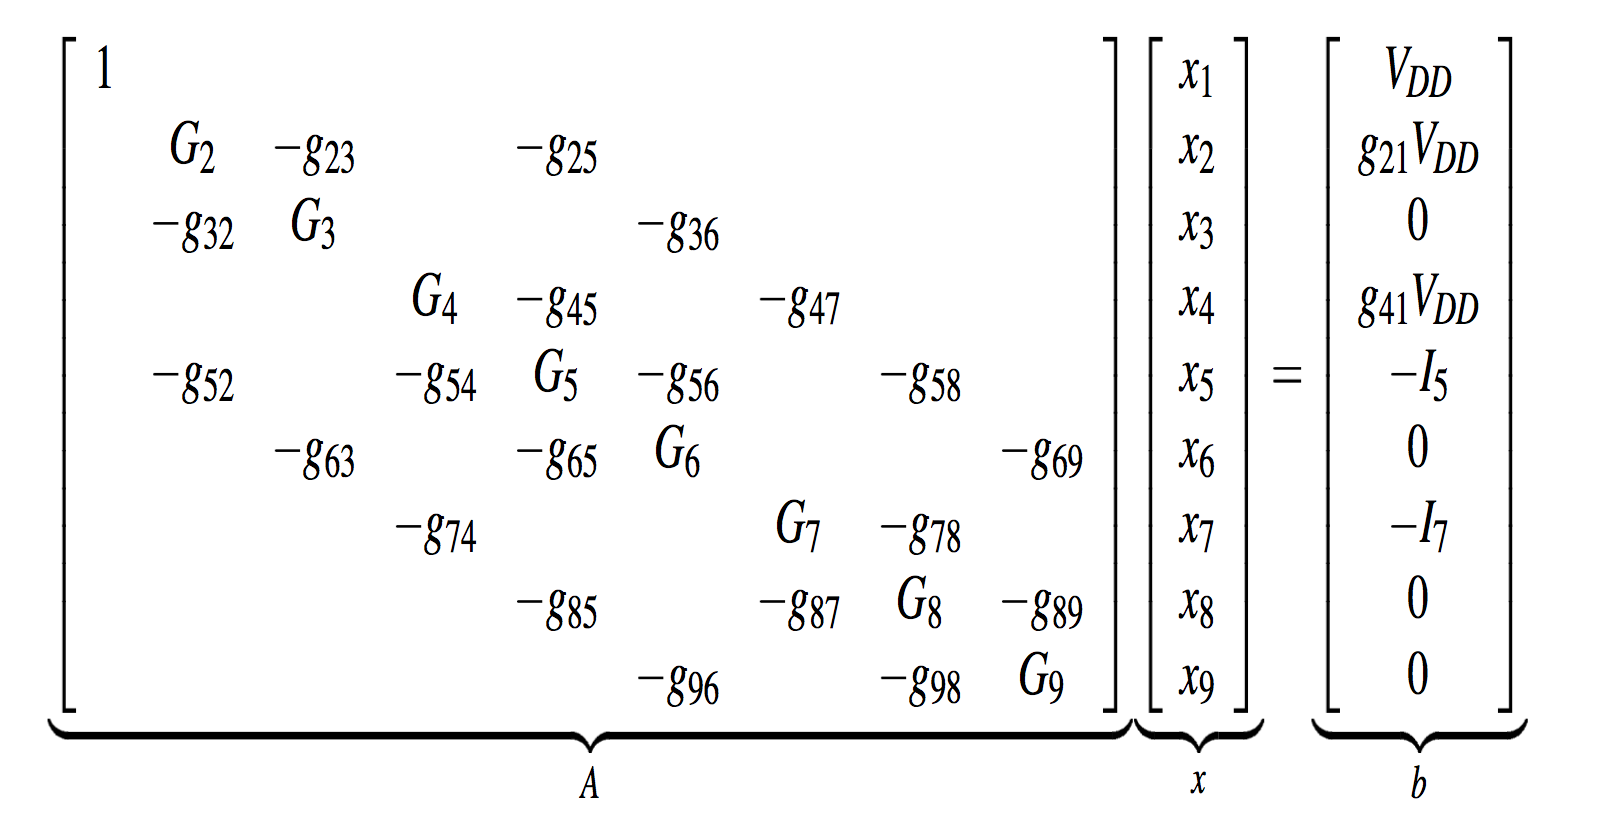
\includegraphics[height=5cm]{a5}
  \caption{变形后的线性方程系统}
  \label{fig:a5}
\end{figure}

我们通过将这种变形的方法应用于上述的3x3网格示例来说明。 节点1具有电压源,因此我们用节点1处的KVL方程代替节点1处的KCL方程。 所得到的系统如图\ref{fig:a5}所示。

观察到右侧也被改变了,产生了新的向量$b$。 很明显,得到的矩阵$A$仍然是对称的;进一步,也是对称正定的。 为此,先注意到$\forall i, |g_{ij}|=|g_{ji}|$。结合\ref{eq:eq3}中的结果,可以得到:
\begin{align}
|G_i| = \sum_{j\in N_i} |g_{ij}|+C_i/h=\sum_{j\neq i}|g_{ij}|+C_i/h\geq \sum_{j\neq i}g_{ij} \quad \forall i
\label{eq:eq4}
\end{align}
式\ref{eq:eq4}适用于每个节点$i$,等效于系统矩阵$A$的每一行。这表明变形后的矩阵$A$是对角占优的,并且已经指出$A$也是对称的。 所以,$A$是一个对称和正定矩阵[9]。 事实上,$A$是M-矩阵[10],因为它满足以下条件:
\begin{enumerate}
\item $a_{ii}>0 \quad \forall i$
\item $a_{ij}\leq 0 \quad \forall i\neq j$
\item $a_{ii}\geq \sum_{j\neq i}|a_{ij}| \quad \forall i$
\item $a_{ii}>\sum_{j\neq i}|a_{ij}| \quad \exists i$
\end{enumerate}
其中$a_{ij}$是矩阵$A$第$i$行第$j$列的元素。所以,在剩下的篇幅里,我们会利用$A$是一个非奇异的$M$矩阵的性质。

\section{多重网格方法}

在精心设计的供电网格中,电阻远远小于等效吸收电阻,因为电网需要为所有的漏极提供稳定的电压。 这将导致局部电力干扰,将被扩散到比引起干扰的区域大得多的区域上。 这种扩散导致空间平滑的电压分布,并且是的我们的对供电网格的解决方案可以利用这种平滑度来加速解决过程。

此外,我们注意到,电网分析会产生一个与二维抛物线偏微分方程(PDE)的有限元离散化相似的线性方程组。 这促使我们将电网问题视为连续PDE的离散化,其中需要在空间固定的点解出所需值。 因此,解决PDE的有效方法值得考虑作为电网问题的潜在解决方案。

近年来,多重网格方法(MG)已经成为解决平滑PDE的标准解法[11],[12],[13]。 多重网格涉及两个基本操作:i)松弛操作和 ii)粗网格校正。松弛操作涉及运行迭代求解器的几次迭代,以平滑误差分量;也就是减少高频误差分量。 另一方面,粗网格校正涉及将问题映射到较粗的网格,在较粗的网格上解决问题,然后将解决方案映射回原始网格。 这两个相辅相成的步骤一起提供了一种解决PDE的有效技术。 因此,在本文中,我们认为可以把它用于电网分析中。

虽然经典的迭代方法由于网格维度增加(等效的网格间距减小)而收敛速度大大降低时,但是多网格性能并不能确定。 事实上,已经证明多网格具有最佳的性能,因为可以用O$(n)$复杂度来解决$n$个方程的系统。多重电网技术 不仅是最优复杂度的,而且所涉及的常数都足够小,让多重电网优于其他方法[13]。 我们应该在这里指出,多重网格方法属于像Jacobi和Gauss-Seidel这样的迭代求解器类别,而不是像高斯消除那样的直接求解器。

我们已经提到,经典迭代方法的分析与对多重网格很有关系。 所以我们将从对经典迭代方法的简要分析开始。 给定线性系统$Ax = b$和初始猜测$x_0$,迭代方案涉及如下:
\begin{align}
\hat{x}^{k+1}=\hat{x}^{k}+M^{-1}(b-A\hat{x}^k)
\end{align}
其中$k$是迭代的当前次数,$\hat{x}^k$是第$k$轮迭代后的对解的估计值。对于$M$,它是一个易于求解的矩阵,使得$M^{-1}\approx A^{-1}$。

令$e = x-\hat{x}$为精确解$x$与近似解$\hat{x}$之间的差。 可以看出,误差可以表示为低频和高频傅里叶模式的线性组合[11]。 此外,经典迭代法的分析导致以下观察[11],[15]:
经典迭代方法有效地降低了高频误差分量,但在降低低频误差分量方面效率不高。

为了避免经典方法的局限性,多重网格方法由两个互补的部分组成:1) 松弛操作,可以减少高频误差;2)粗网格修正,可以减少低频误差。

\begin{figure}[H] % use float package if you want it here
  \centering
  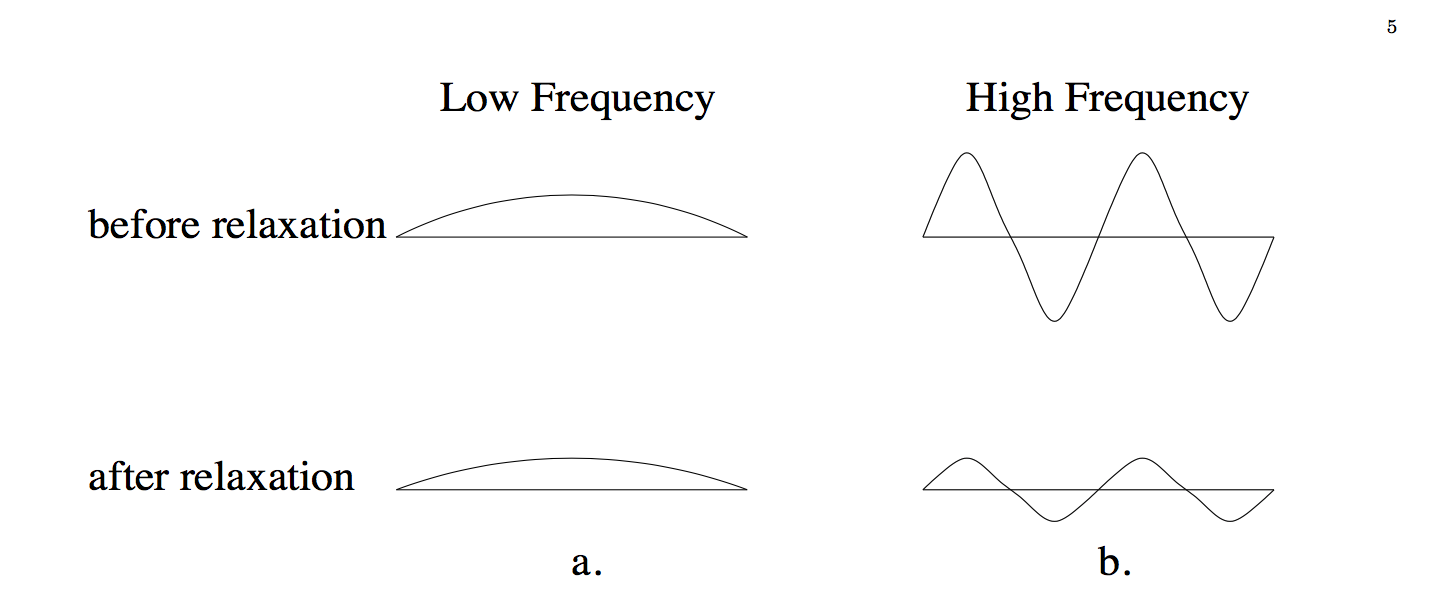
\includegraphics[height=6.5cm]{a6}
  \caption{迭代方法的松弛效果}
  \label{fig:a6}
\end{figure}

松弛操作涉及到经典迭代求解器的几次迭代。从观察结果可以看出,经典的迭代方法是良好的平滑器,如图\ref{fig:a6}所示[15]。另一方面,粗网格校正将问题映射到较粗的网格,解决映射问题,并将得到的解映射回到精细的网格。两个网格(细和粗)之间通信所需的关键工具是网格间转移子,分别是网格限制子和网格延长子。粗网格校正的一个直观的动机是粗网格的解决方案通常为细网格上的迭代求解器提供了良好的初始猜测,从而能加速收敛。这种方法的另一个动机是,如图\ref{fig:a7}所示,细电网$\Omega^h$的低频误差分量在粗网格$\Omega^{2h}$出现更多的振荡。所以应在较粗的网格上进行松弛操作,减少这些误差成分。

\begin{figure}[H] % use float package if you want it here
  \centering
  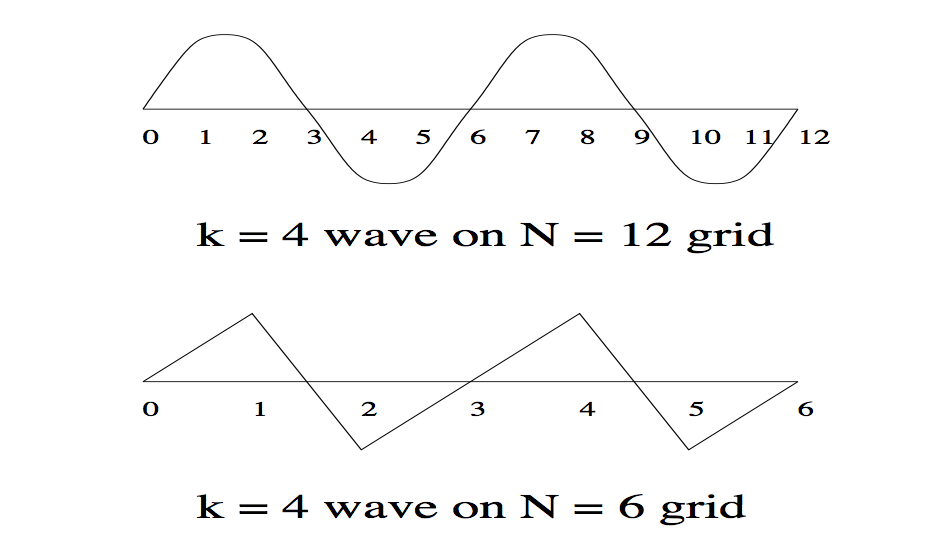
\includegraphics[height=6cm]{a7}
  \caption{迭代方法的松弛效果}
  \label{fig:a7}
\end{figure}

多重网格技术的工作如下[11]。 从精细网格开始,进行几个松弛步骤应用以减少误差中的高频部分。 然后误差中的低频部分通过粗网格校正也得到了降低。 这产生了下面的这个高效率的算法,我们称之为V-循环多重网格方法。 在下文中,$R_h^{2h}$和$P^h_{2h}$分别对应于限制操作子和延长操作子。 另一方面,$V^h$表示V-cycle算法;并且用$h$定义V-cycle算法被调用的深度。 $v_1$和$v_2$是要执行的迭代次数,是常数。 这些常数是依据经验选择的,通常是2或3。

\begin{align*}
\hat{x}^h \leftarrow V_h(\hat{x}^h, b^h)
\end{align*}
\begin{enumerate}
\item 用初始解$\hat{x}^h$对$A^hx^h=b^h$进行$v_1$次迭代松弛操作;
\item 如果目前的$\Omega^h$是可以容许的最粗的网格,那么去第四步;否则令$b^{2h}\leftarrow R_{h}^{2h}(b^h-A^h\hat{x}^h)$,$\hat{x}^{2h}\leftarrow 0$,$\hat{x}^{2h}\leftarrow V^{2h}(\hat{x}^{2h}, b^{2h})$;
\item 修正:$\hat{x}^{h} \leftarrow \hat{x}^h + P^h_{2h}\hat{x}^{2h}$
\item 用初始解$\hat{x}^h$对$A^hx^h=b^h$进行$v_2$次迭代松弛操作;
\end{enumerate}


\section{供电网格中的多重网格分析方法}

在这一节中,我们讲讲述这个供电网格分析的新方法的各种细节。这个技术使用了多重网格理论的一般思想。然而,它独特地瞄准着供电网格问题的细则,从而产生了一个更高效的算法。

供电网格分析包含三步:1)对供电网格、电流源、漏极进行建模;2)使用改进的节点分析法(MNA)对线性系统$Ax=b$进行形式化;3)对$Ax=b$进行求解,从而得出供电网格所有节点的电压降。

前面已经讨论了对供电网格,电流源和漏极进行有效分析时模型建立的必要性。 此外,通过应用改进的节点分析(MNA),线性系统$Ax = b$的公式已经在前面已经说明过了。 因此,仍然要讨论的是如何有效地解决所得到的线性系统$Ax = b$。

如第三节所述,电网问题最初是一个离散的问题,因此启发我们使用代数多重网格的算法。 然而,成功应用代数多网格需要定义一个良好的插值算子。 这规定了一个满足以下要求的网格缩减(粗化)机制:

\emph{对于每个被删除的节点$i$,所有强连接到$i$的节点$j$要么被继续保留,要么强制连接到至少一个节点$k$,其中$k$被保留并且强连接到$i$。}

满足上述要求可能导致网格缩减的效率低下。 具体来说,所得到的粗化的网格可能不够粗糙;也就是说,网格缩减只能移除少量的节点。 这就意味着算法效率不高,在CPU时间和内存方面花销很高。 因此,为了避免算数多重网格的限制,我们提出了一种类似于使用标准多重网格的网格缩减算法的算法。 然而,由于典型的供电网格可能是不规则的,我们的算法被设计为能有效地处理供电网格的不规则性,并且在每次迭代时产生显着减小的较粗网格。

一旦网格被缩减,我们提出的方法定义了插值算子,以满足代数多重网格方法的要求。 也就是说,插值算子被定义为使得不能很好地减少的误差分量位于其范围空间中的算子。假设插值运算符满足:
\begin{align}
e^h_i & =e^H_i &\text{如果 }i\text{ 被保留 或者} \\
e^h_i & =\sum_{j\in N_i} \frac{|a_{ij}|}{a_{ii}} e^H_j &\text{如果 }i\text{ 被移除}
\end{align}
其中$h$和$H$分别表示细网格与粗网格。

这个定义可以保证误差在于插值算子所定义的范围空间内,因为$e^h = P_H^he^H$。 注意如果$|a_{ij}|/a_{ii}$很小,那么节点$j$的效果可以忽略不计。 也就是说,将已删除的节点$i$的电压与强连接到$i$的那些节点进行插值是足够的。 基于此,我们从去除的节点$m$与$m$强连接的节点的电压进行插值。 由于网格的几何形状是已知的,因此可以容易地识别出与$m$强连接的且仍保留着的节点。 通常来说,这些将是$m$的几何邻居和/或其这些邻居对应的邻居。

因此,提出的方法结合了标准与代数这两种多重网格技术的优点,同时避免了它们的局限性。 此外,所提出的方法与常规多重网格相比还有另一个显着的优点。 如前所述,多重网格包含两个主要部分:松弛(或平滑)操作和粗网格校正。 松弛操作的作用基本上是平滑误差分量,而粗网格校正的作用是近似估计那些平滑的误差分量。 然而,在电网中,误差分量通常是平滑的,因为供电网格被设计成在网格上具有平滑的电压变化。 因此,在解决电网问题时,可以忽略多重网格的松弛步骤,仅集中在粗网格校正步骤上。 这正是我们提出的方法所做的,下面的实验结果表明,这种假设带来了显着的加速,同时只引入了非常小的误差。

假设平滑的电压变化,忽略松弛步骤,我们提出的方法属于直接求解器的类型,而不是基于迭代求解器的多重网格技术。 当进行瞬态分析时,这会导致算法获得进一步加速。 给定一个初始电网$\Omega^h$及与之相关的线性系统$A^hx^h = b^h$,提出的方法可以总结如下:
\begin{enumerate}
\item 在细网格上进行缩减算法,产生一个粗网格$\Omega^{2h}$;
\item 定义插值操作子$P_{2h}^h$;
\item 如果$\Omega^{2h}$不够粗,那么先把$\Omega^{2h}$拷贝到$\Omega^h$上,然后更新插值操作子$P_{2h}^h$,然后返回第一步进行递归;另一方面,如果$\Omega^{2h}$足够粗,那么把问题映射到粗网格上:$A^{2h}=(P_{2h}^h)^TA^hP^h_{2h}$ 并且
$b^{2h}=(P^h_{2h})^Tb^h$,然后在粗网格上求解$A^{2h}x^{2h}=b^{2h}$,最后把解映射回细网格中:$x^h=P^h_{2h}x^{2h}$。
\end{enumerate}

注意到,对网格的缩减标准是是用户自定义的。 网格粗略足够的标准涉及程序精度和运行速度之间的权衡。 供电网格越粗,解决方案越快,但精度越低。 通常,足够粗的网格指的是问题的大小足够小以至于能快速有效解决的网格。 在我们的实现中,四个级别的供电网格缩减(根据经验)足以产生可以有效解决的缩减系统。

在本节的剩下部分中,我们将关心粗网格校正过程,一旦选择了粗化策略并定义了插值算子,这一过程就被完全确定了。 我们定义和讨论了网格缩减算法。 然后我们将说明插值算子是如何定义的。 最后,讨论了使用多重网格技术进行瞬态分析的优点。

\subsection{网格缩减}

\begin{figure}[H] % use float package if you want it here
  \centering
  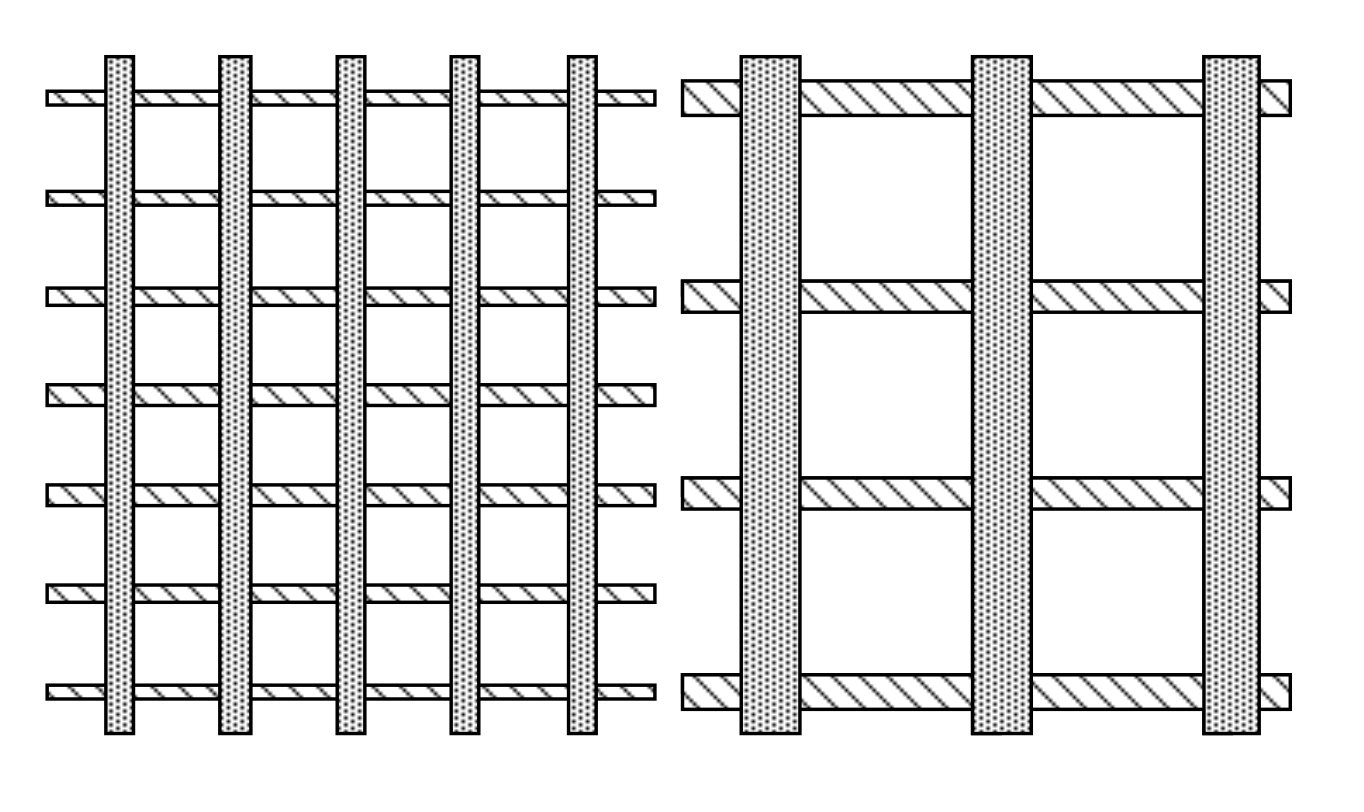
\includegraphics[height=6cm]{a8}
  \caption{供电网格的多种解析度}
  \label{fig:a8}
\end{figure}

一种有效的供电网格缩减方法是跳过所有其他导线,导致如图\ref{fig:a8}所示的情况。 然而,典型的供电网格可能是不规则的,即不同的边缘可能具有不同的长度和不同的间隔距离。 因此,网格缩减算法应该具有缩减任何一般网格的功能通用性。 此外,该算法应该保持原始的网格结构,使其可以被递归地应用,直到产生足够粗的网格。

网格缩减算法的主要目标是移除尽可能多的节点,同时保持通过插值估计被去除节点的电压的能力。 该算法将精细网格$\Omega^h$和要保留的节点列表作为输入,并输出具有较少数量节点的缩减网格$\Omega^{2h}$。 保留节点的列表应由用户感兴趣的特定节点组成,但我们的技术自动生成包含电压源所在的节点和角落节点的列表。


\begin{figure}[H] % use float package if you want it here
  \centering
  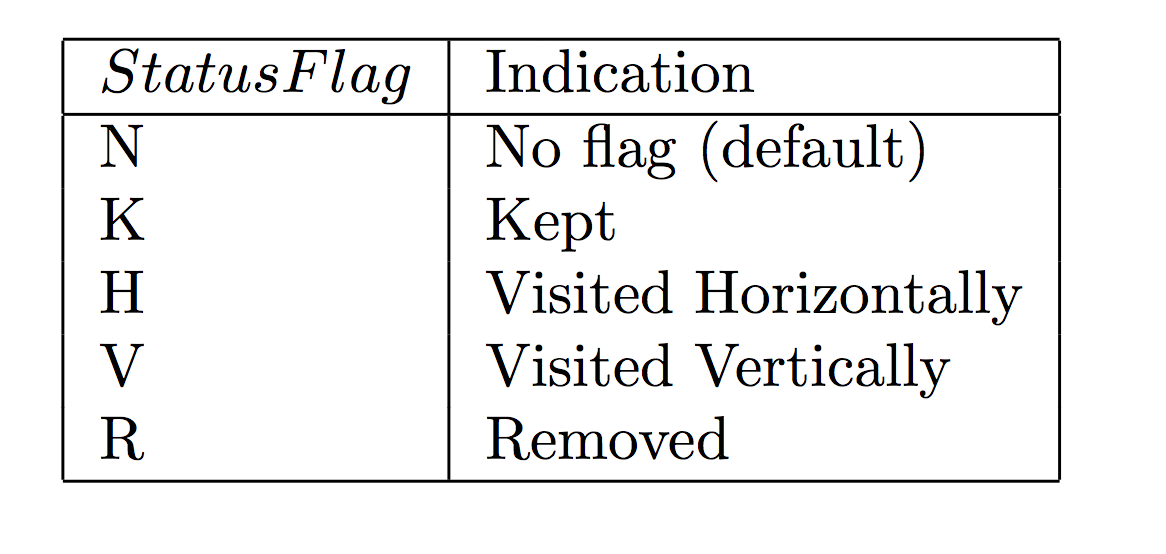
\includegraphics[height=3cm]{t1}
  \caption{状态标记的定义}
  \label{fig:t1}
\end{figure}

该算法利用表\ref{fig:t1}中说明的某些状态标志来确定节点是保留还是移除。 此外,这些标志指示如何从被保留的邻居插值获得已删除节点处的电压。 网格缩减算法重复使用所谓的节点更新操作,操作定义如下:从该节点开始沿着水平(垂直)方向,并用H(V)标记所有访问节点。 同时被水平和垂直访问的节点(标记为H和V)被标记为保留。 该算法由三个步骤组成,如下所述:
\begin{enumerate}
\item 第一步:对所有\emph{保留}节点进行\emph{更新操作};
\item 第二步:对于所有H(V)节点,标记它为R,表示移除;然后标记它沿着同一行(列)邻居为\emph{保留}并对其进行\emph{更新操作};如果一个节点没有被标记(N),那么标记它为移除(R),标记它的对角线上的邻居为\emph{保留}并进行\emph{更新操作};
\item 第三步:被保留的节点的电压值与它在粗网格上计算得来的值相同。一个H(V)节点(也就是被移除节点)的电压值由它的邻居(沿行或列方向)插值而来。标记为N的节点的电压值从它的被标记为\emph{保留}的对角邻居插值而得到。
\end{enumerate}
节点X的对角线邻居被定义为通过从水平方向首先前进一步,然后再垂直地走一步;或先垂直地然后水平地走一步而达到的那些节点。 例如,如果节点Y是节点X的上邻,则Y的左右邻居是X的对角邻居。

\begin{figure}[H] % use float package if you want it here
  \centering
  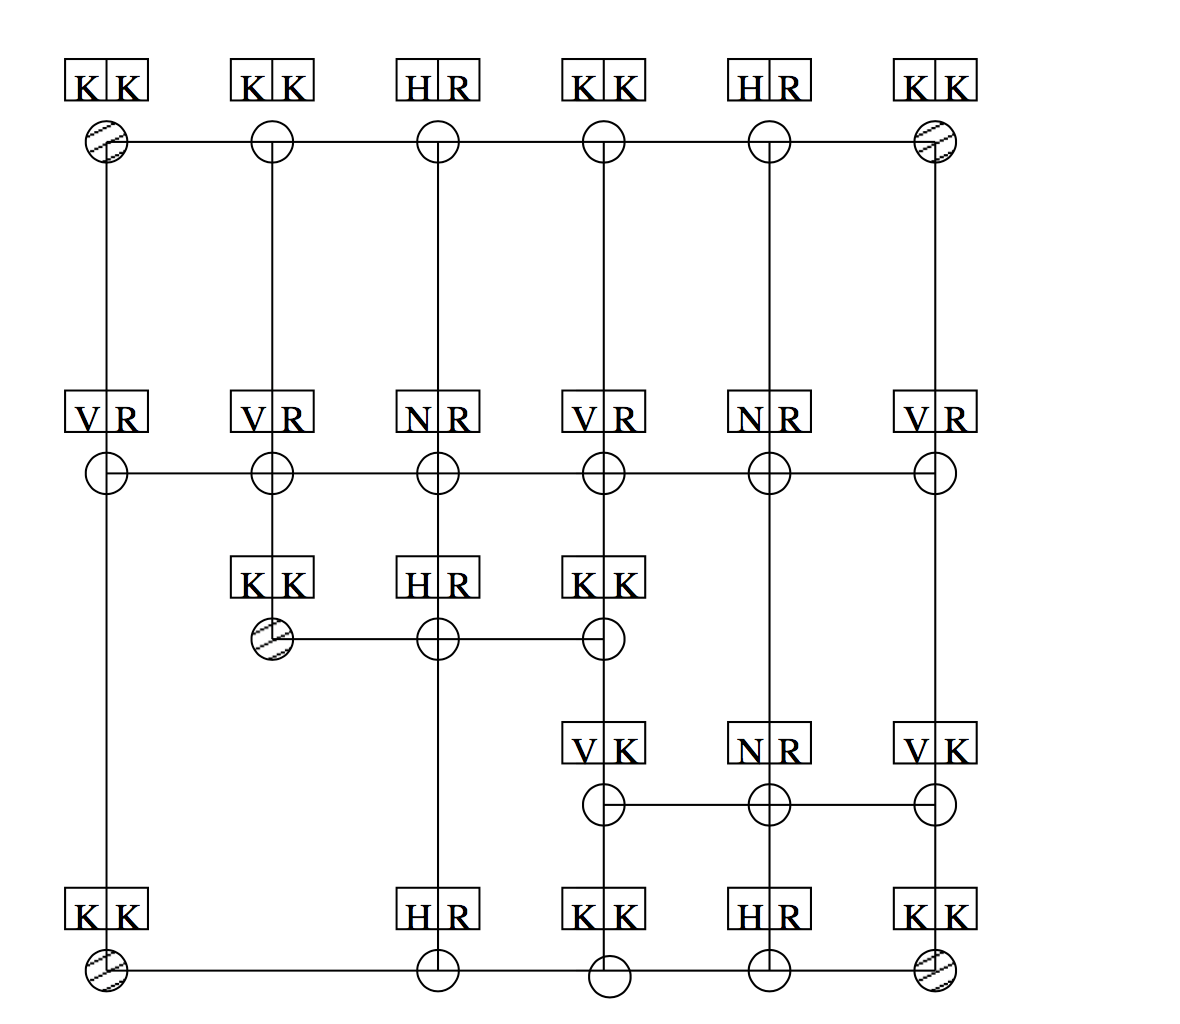
\includegraphics[height=9cm]{a9}
  \caption{对不规则网格的缩减示例}
  \label{fig:a9}
\end{figure}

该算法由图\ref{fig:a9}所示的不规则网格$\Omega^h$表示,其将被缩减而得到网格$\Omega^{2h}$。 在实施供电网格缩减算法时,网格节点从上到下、从左到右按顺序排列。 然而,值得注意的是,这不足够强大以处理任何的节点序列。

一开始,所有节点的默认状态为N,除了应保留的节点。 在这个例子中,被保留的节点将是网格的所有角落节点(图\ref{fig:a9}中的虚线节点)。 由两个字符组成的标签与网格的每个节点相关联。 左边字符表示第一次通过后节点的状态,右边字符表示第二次通过后节点的状态。

如图\ref{fig:a9}所示,在第一步完成之后,由至少一个保留节点组成的行或列的末端被标记为保留。 基于边缘是水平还是垂直的,边缘上的剩余节点用H或V标记。 注意到一些节点仍然具有N的状态标志,这表示在第一次通过期间这些节点未被访问。 然后在第二步完成之后,保留具有K标志的节点,而具有R标志的节点被去除,从而产生较粗的网格$\Omega^{2h}$。

\begin{figure}[H] % use float package if you want it here
  \centering
  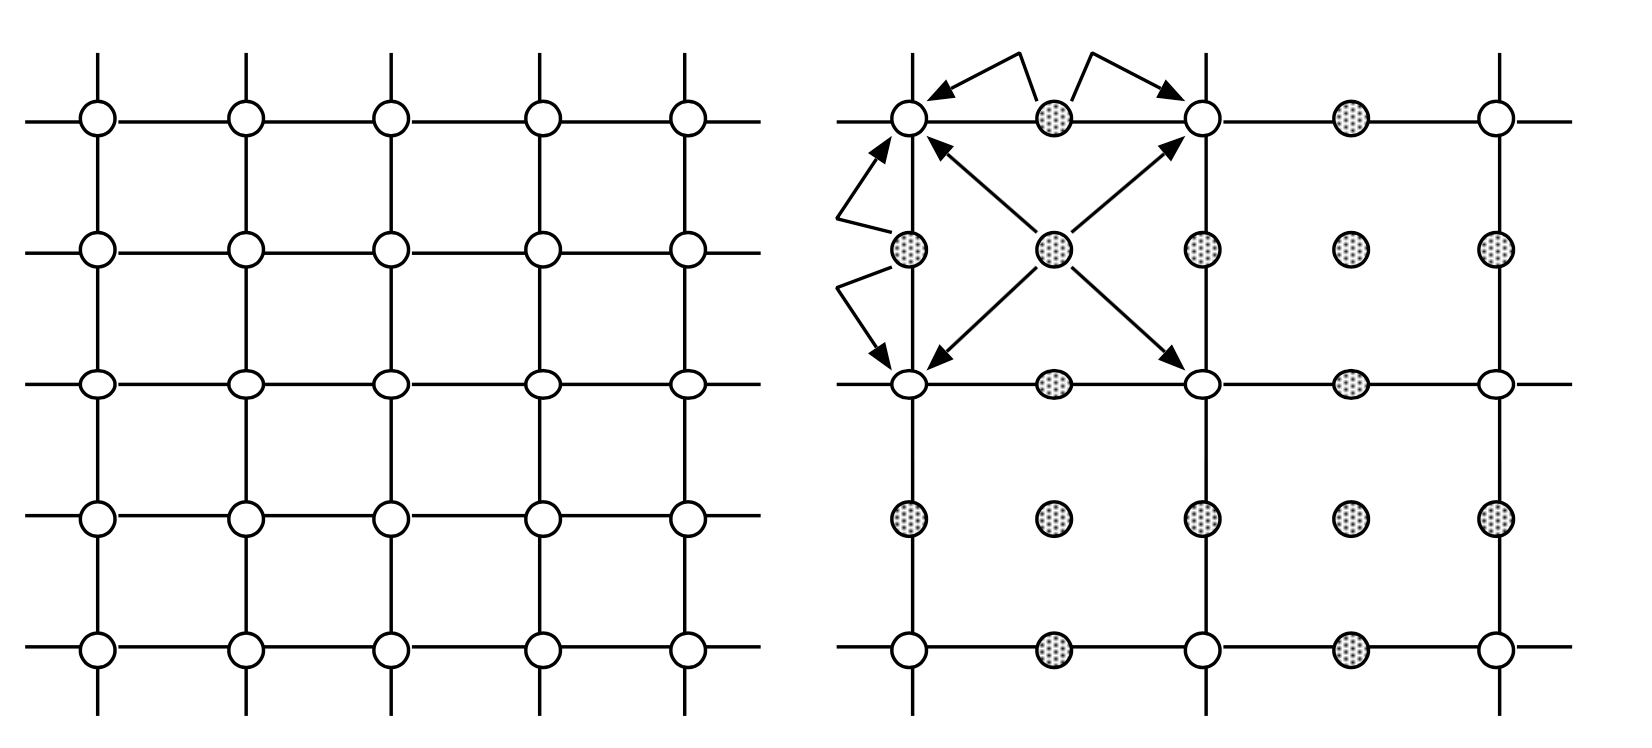
\includegraphics[height=7cm]{a10}
  \caption{基本的缩减操作}
  \label{fig:a10}
\end{figure}

最后,我们指出,如果原始网格是规则的,那么算法是最优的。 也就是说,它导致如图\ref{fig:a10}所示的例子中的节点数量达到最大的缩减。在这种情况下,每次网格缩减操作能产生一个线性方程组,其未知数数量减少约4倍,运行时的CPU时间减少约8倍。

\subsection{插值操作}

AMG的插值操作子应该使得:被去除的节点$i$的电压与和$i$强连接的那些被保留的节点的电压相关联。 通常来说,当$|a_{ij}|/\max_{l\neq i}|a_{il}|\geq \theta$,其中$0\leq \theta \leq 1$(在实践中$\theta$通常被选取为$0.25$)时,AMG会考虑两个节点$i$和$j$之间有强连接。 通过这种插值操作子的选择,粗网格校正可以有效地减少误差。

在我们的缩减算法中,状态标志指示删除的节点的哪些邻居将用于插值,而这取决于它们被保留并且与被去除的节点$m$强连接。 对于插值权重,可以通过考虑节点间的电导值来获得。 因此,如果用节点$A$和$B$处的电压插值得到被去除节点$m$处的电压,则他们的(线性)插值函数INT()定义为:
\begin{align}
V(m)=\text{INT}(V(A),V(B))=a_0V(A)+a_1V(b)
\end{align}
其中$a_0=\frac{g_{mA}}{g_{mA}+g_{mB}}$,并且$a_1=\frac{g_{mB}}{g_{mA}+g_{mB}}$。在这里,$g_{mA}$表示节点$m$与节点$A$之间的电导,$g_{mB}$表示节点$m$与节点$B$之间的电导。注意到我们选取插值权重的方法来源于代数
多重网格中的类似方法。为了说明,考虑一个被取出节点$m$,它的电压会从保留节点$A$与$B$中插值而得来。代数多重网格方法使用下面的插值方法:
\begin{align}
V(m)=\frac{|a_{mA}|}{a_{mm}}V(A)+\frac{|a_{mB}|}{a_{mm}}V(B)
\end{align}
其中$a_{mA}$是矩阵$A$中与$m$与$A$关联的元素,$a_{mB}$是矩阵$A$中与$m$与$B$关联的元素。至于$a_{mm}$,一种代数多重网格中的方法是把它定义为矩阵中$m$对应的对角元素。另一种多重网格中的方法是定义为:$a_{mm}=|a_{mA}|+|a_{mB}|$。在供电网格
方法中,$|a_{mA}|=g_{mA}$,且$|a_{mB}|=g_{mB}$,这说明我们的插值方法来源于代数多重网格方法。

\begin{figure}[H] % use float package if you want it here
  \centering
  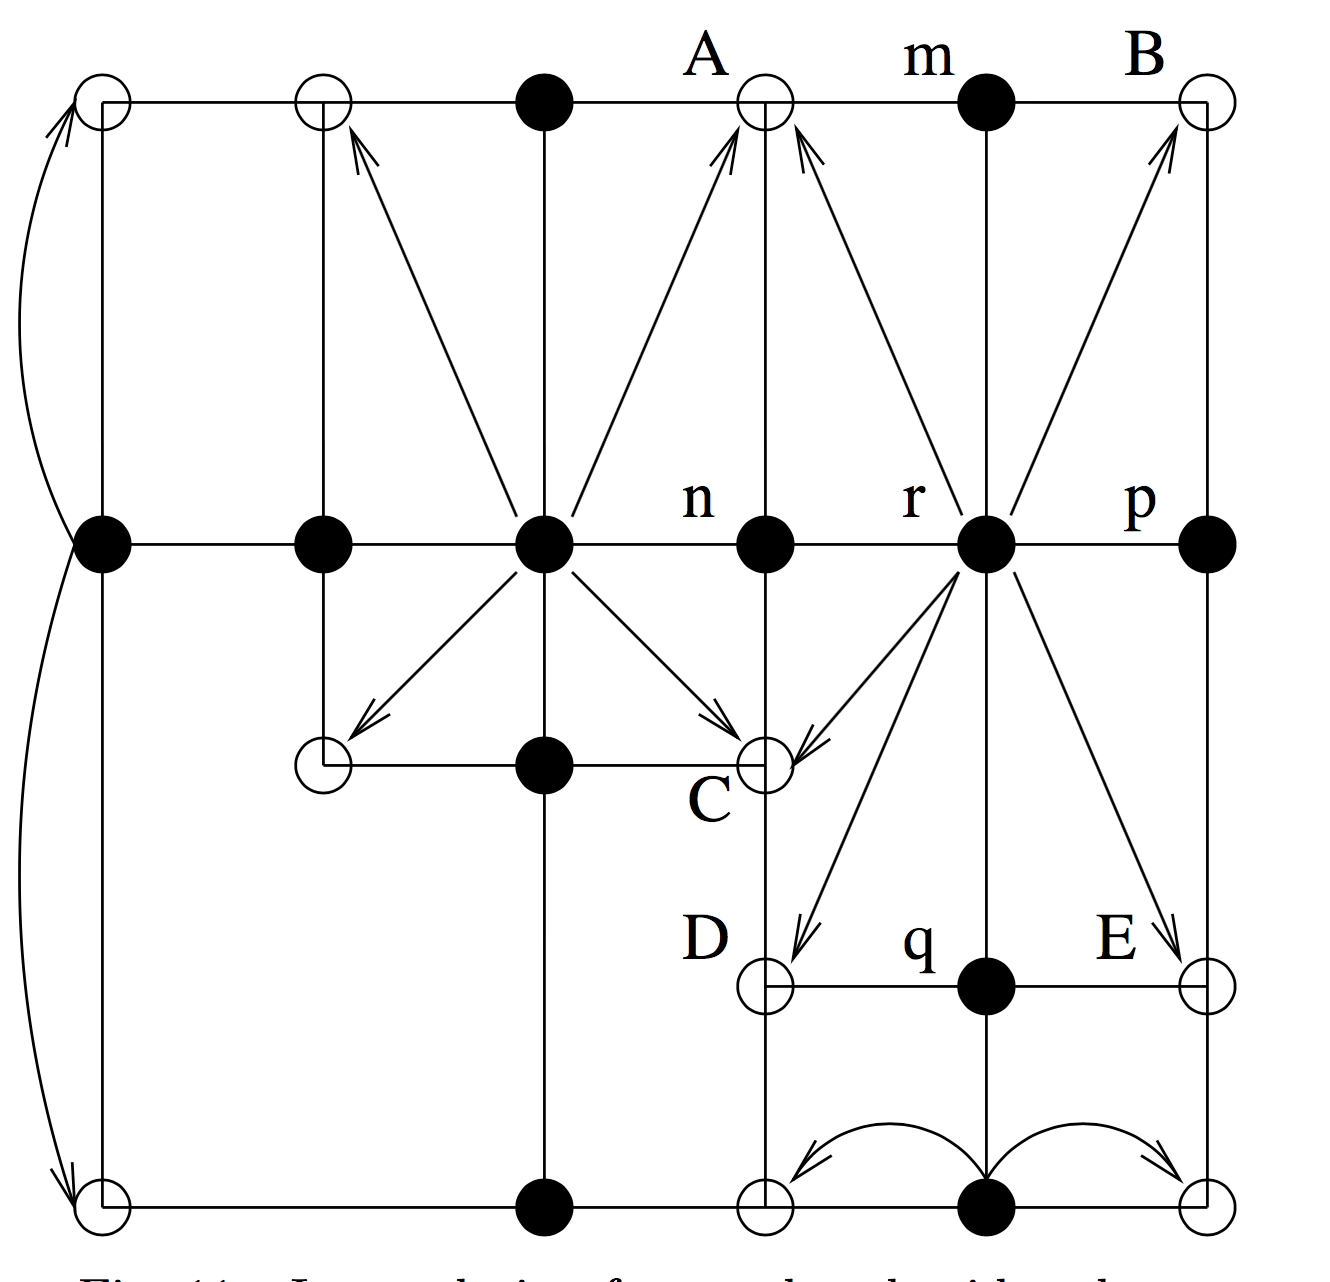
\includegraphics[height=7cm]{a11}
  \caption{在缩减网格中进行插值操作}
  \label{fig:a11}
\end{figure}

然而,这还不是全部。回想一下,我们的供电网格缩减算法与代数多重网格缩减方法不同;它实际上是基于标准多重网格算法的缩减算法,它只使用了几何信息,并删除尽可能多的节点。因此,有可能遇到被移除节点$i$的与其强连接的所有节点也被删除的情况。为了说明这一点,考虑图\ref{fig:a11},其中实心节点指示被去除的节点,空心节点指示保留的节点。在这个例子中,我们假设每个水平或垂直连接都代表一个强连接,但由两个或更多个连接分开的节点间并没有强连接。这种情况是供电网格的典型情况。因此,r与m强连接,m与B强连接,但r和B不连接。这种类似于B的节点,与r之间没有强连接但是通过两个强连接能与r有关系的节点,我们称它们与r\emph{二度强连接}。我们的网格缩减将删除节点r,以及强烈连接到它的所有节点,m,n,p和q。然而,可以发现,我们的算法保证,如果删除节点i,则保留与i强连接的一些节点,或者保留与i\emph{二度强连接}的一些节点。因此,在我们的插值技术中,如果一个节点的所有强连接的邻居与它一起被去除,我们使用它的\emph{二度强连接}的保留的邻居节点进行插值。这在图\ref{fig:a11}中能清楚地看出。,其中节点r处的电压从\emph{二度强连接}到r的那些节点插值而得到;具体来说,是节点A,B,C,D和E。注意,这种方法保持了有效网格减少的优点,同时满足了良好的插值操作子的要求。

\subsection{实验结果}
本论文所提出的多重网格方法已被实现并集成到用C++编写的线性模拟器中。 本节报告的所有实验结果都是通过在具有2GB RAM并运行SunOS 5.7操作系统的400MHz ULTRA 2 Sun工作站上运行仿真而获得的。

我们通过把算法应用于两个工业中实际的ASIC设计电网分析例子,来说明所提出的技术的实用性和效率。 我们将这些设计称为C1和C2。 C1和C2均为$0.18\mu$的CMOS设计,电源电压为1.8V。对于供电网格来说,该技术需要输入与芯片上不同功率的漏极相关的电流。

根据不同的目标,我们可以使用不同的电流度量进行分析。 例如,虽然峰值电流值是IR降低的一个很好的测量方式,但平均电流值是电磁分析中更好的测量方法。 另一方面,电流波形是瞬态分析中相当合适的电流度量方式。 获得当前感兴趣的电流度量的直接方法是模拟在额定负载和现实切换因素下的功率消耗情况。 这是我们当前用于分析的主要方法。 在我们所有面对直流分析的实验中,我们使用功率消耗器绘制的峰值电流作为我们当前的测量值。 对于瞬态分析,所使用的电流度量是与不同功率的漏极相关的电流波形。

\begin{figure}[H] % use float package if you want it here
  \centering
  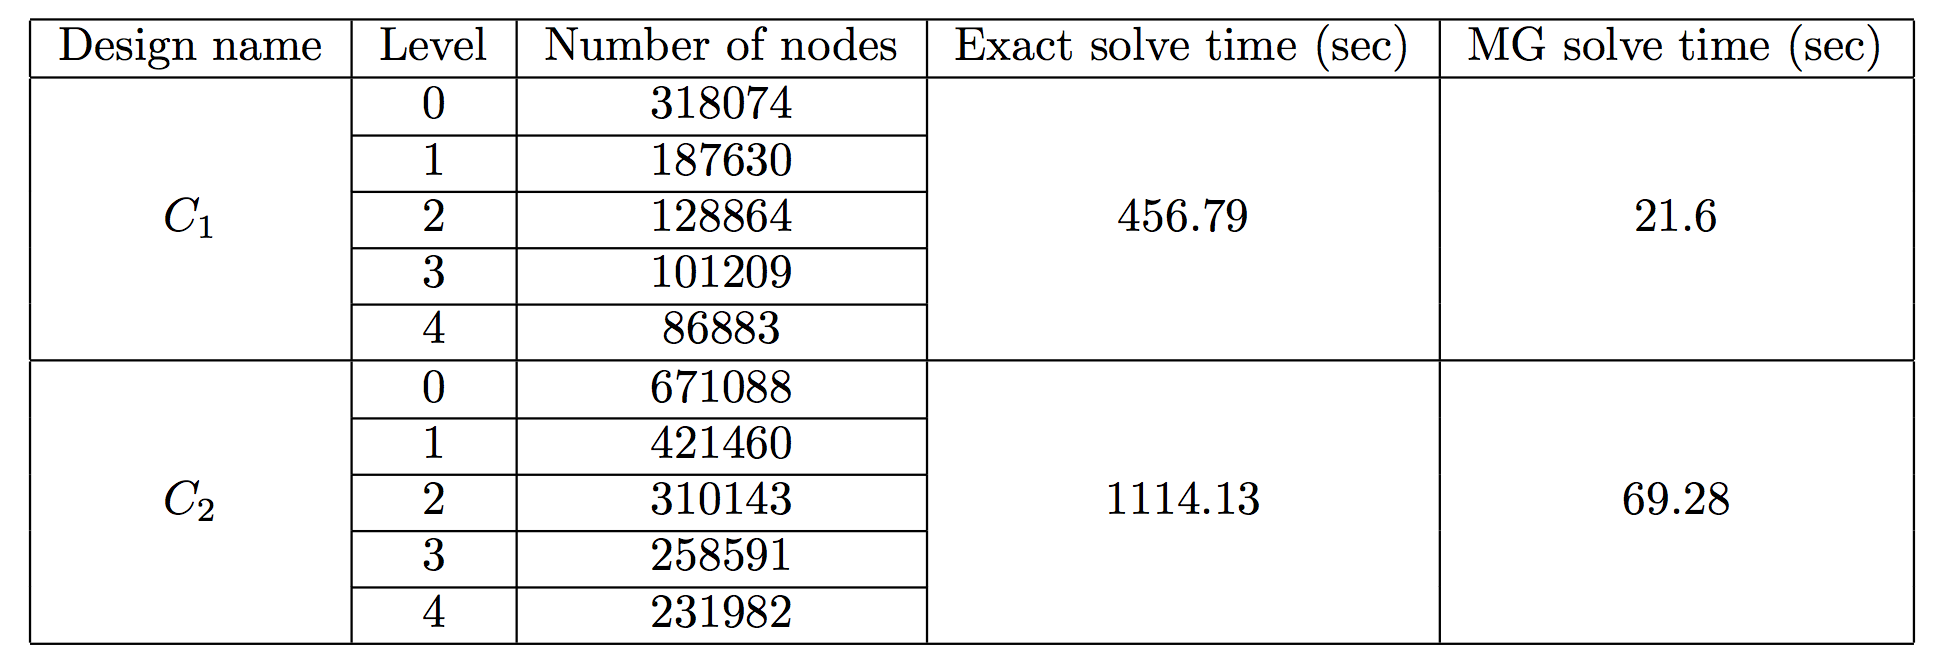
\includegraphics[height=5cm]{t2}
  \caption{使用直接求解器与多重网格技术后的网格缩减结果及其运行时间}
  \label{fig:t2}
\end{figure}

我们模拟了两种不规则电网的设计C1和C2。 应用了几个网格缩减之后,问题相应地映射到较粗的网格(如前所述,不断进行网格缩减操作,直到网格如用户所指定的那样粗糙)。 表\ref{fig:t2}中显示了在指定四个级别的缩减操作时,每个级别的网格节点数。 表中还显示了使用常规直接求解器(如第4列所示)求解给定线性系统以及我们所提出的多重网格式技术(如第5列所示)的CPU时间。 很明显,我们所提出的新技术比传统的仿真快16至20倍。 请注意,实验中使用了相同的直接求解器来解决原始的网格系统以及缩减后的网格系统,从而验证了加速不是由于求解器之间的差别而到导致的。

为了验证我们提出的技术的计算结果的准确性,我们将准确的解与我们的算法返回的估计解相比较。 两个设计C1和C2的不同节点的电压中的相对误差的直方图分别如图\ref{fig:a12}和\ref{fig:a13}所示。

对于设计C1,节点电压误差的分布平均值为$-0.0077\%$,标准偏差为$0.0333\%$。 对于设计C2,误差分布的平均值为$-0.0026\%$,标准偏差为$0.0167\%$。 此外,图\ref{fig:a12}和\ref{fig:a13}还显示了两种设计的所有电网节点的误差在$-1.0\%$至$1.0\%$的范围内。 事实上,设计C1的错误范围从$-0.93\%$到$0.66\%$,而设计C2的误差范围从$-0.30\%$到$1.0\%$。 因此,很明显,我们所提出的技术提供了对于供电网格问题的准确的解决方案,并且比正常求解器有着显著的效率优势。

\begin{figure}[H] % use float package if you want it here
  \centering
  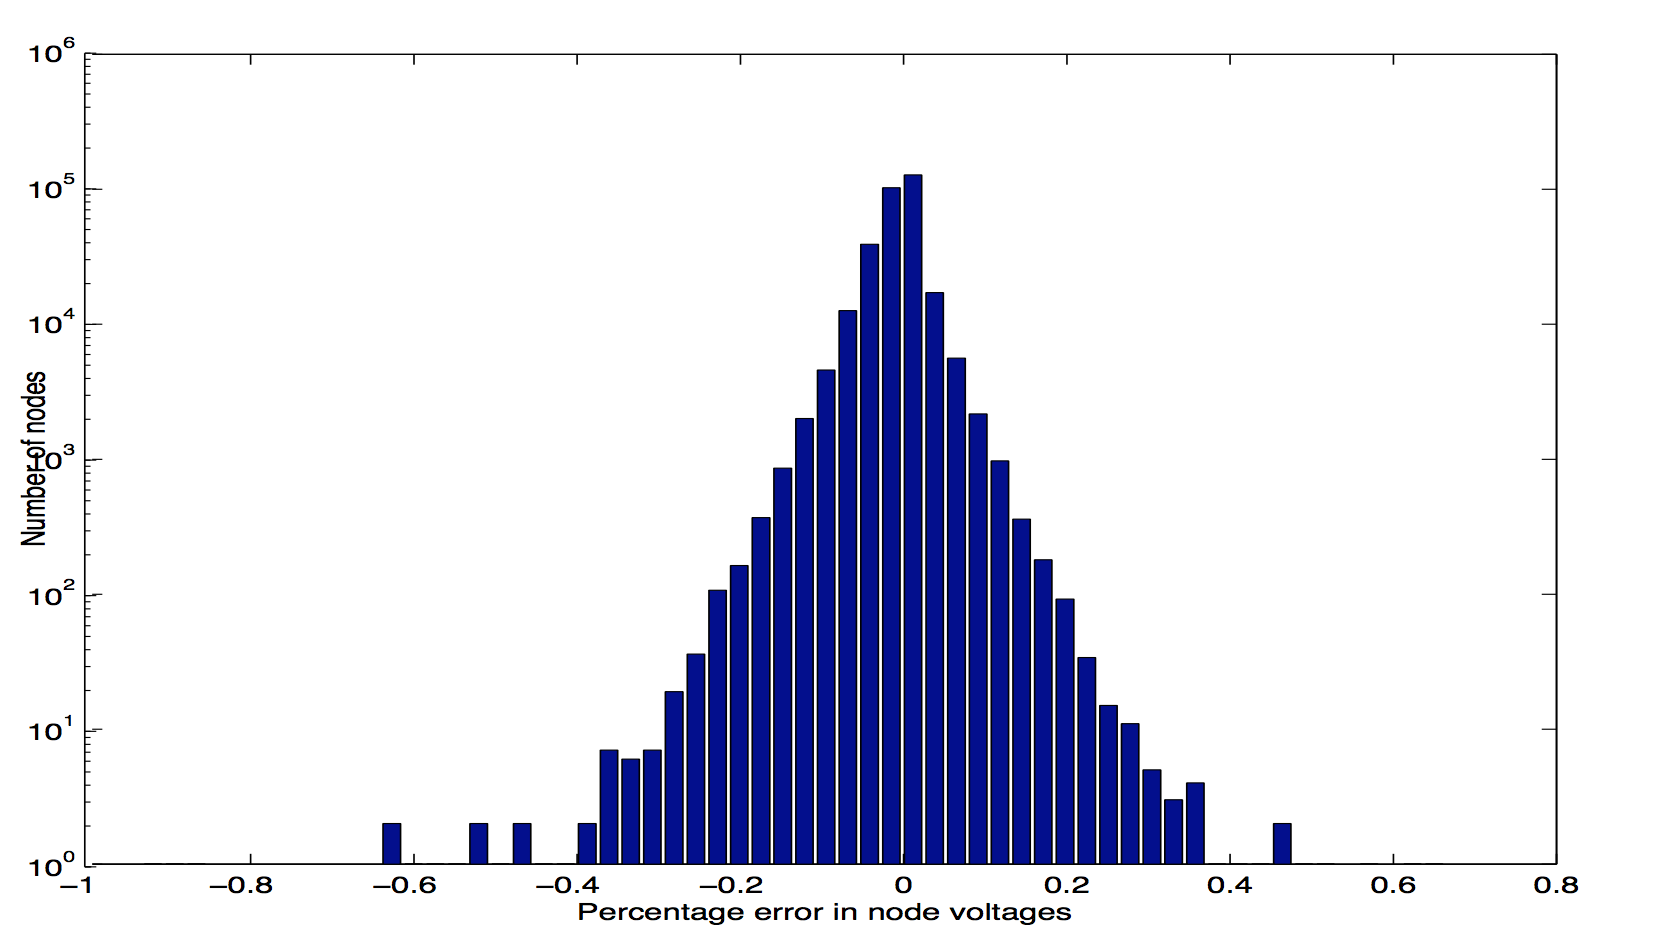
\includegraphics[height=9cm]{a12}
  \caption{C1设计中的节点电压值误差直方图}
  \label{fig:a12}
\end{figure}

\begin{figure}[H] % use float package if you want it here
  \centering
  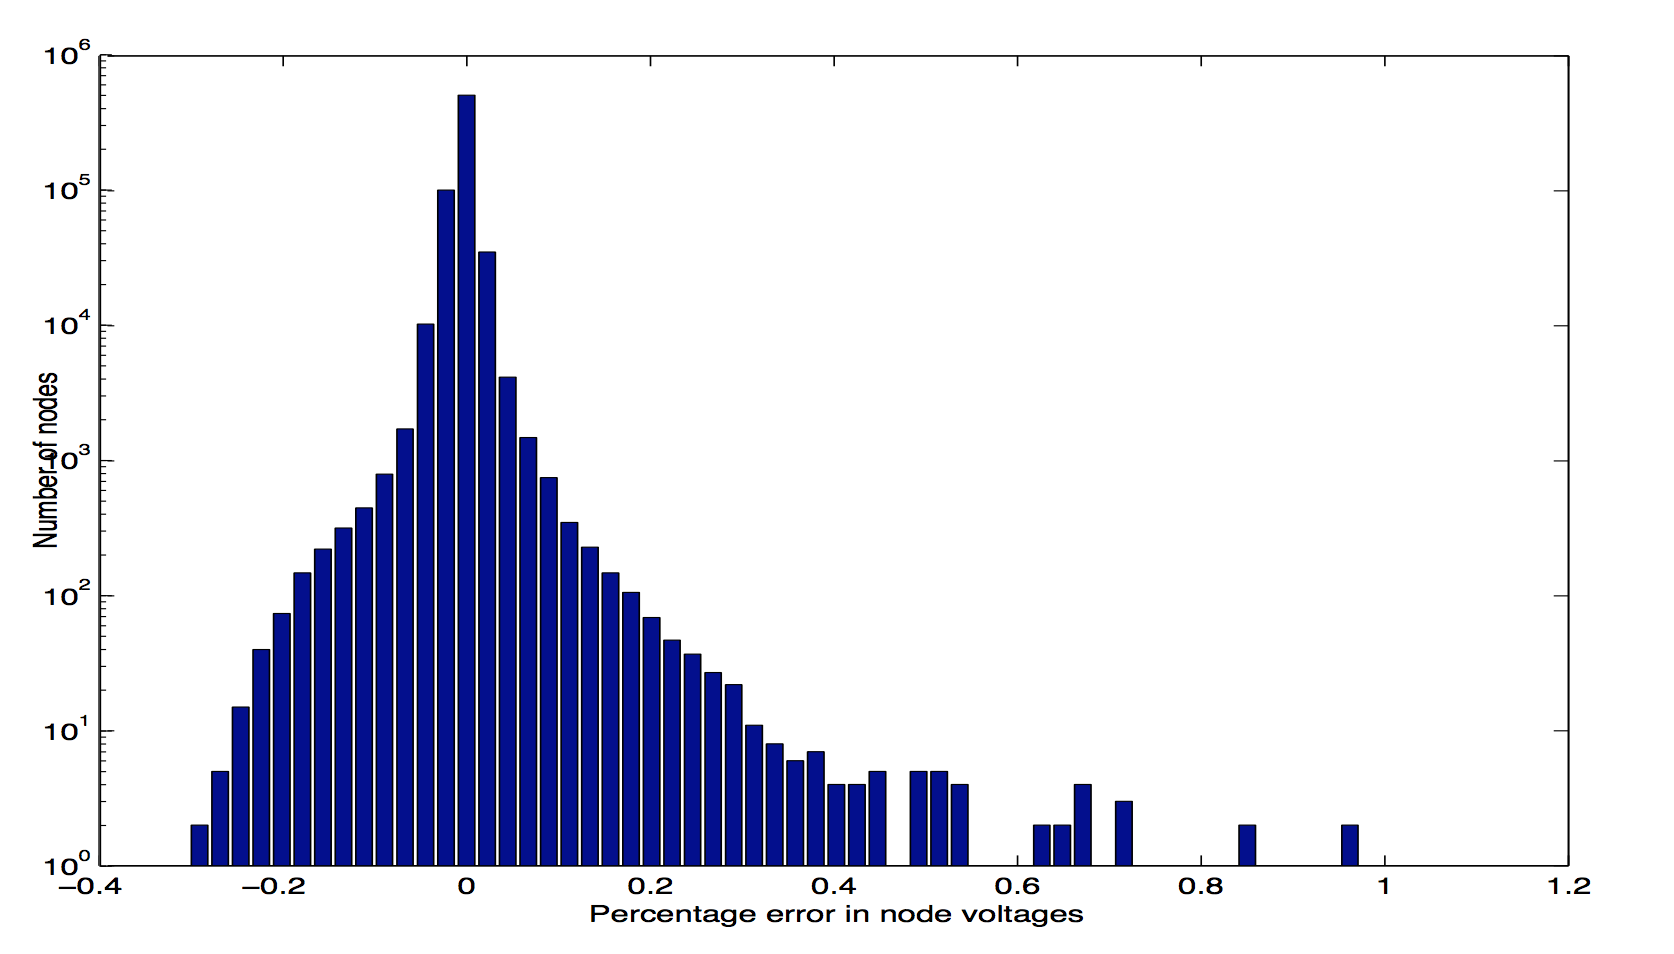
\includegraphics[height=9cm]{a13}
  \caption{C2设计中的节点电压值误差直方图}
  \label{fig:a13}
\end{figure}

如前所述,我们提出的多网格技术在应用于瞬态分析时更为有利。由表\ref{fig:t3}说明,其显示了使用常规求解器和我们的技术来运行两种设计的供电网格的瞬态模拟所需的时间。供电网格的模拟时长为4ns,时间步长为0.4ns。在这两种设计中,我们的技术的加速优势都是明显的。然而,在C2设计的情况下更为显著,原因是由于内存限制,C2设计中我们只能使用迭代求解器来模拟。在这个情况下,对于每个时间步长,迭代求解器总共使用了14.3小时来模拟供电网格。然而,另一方面,我们的技术使用直接求解器来解决网格上的问题。在这个情况下,只需要一个初始矩阵因子分解,并且在剩余时间步长中仅需要前向/后向求解。所以使用我们的多网格技术进行瞬态分析所需的总时间仅为86.36秒,代表瞬态分析的加速比为600倍。

\begin{figure}[H] % use float package if you want it here
  \centering
  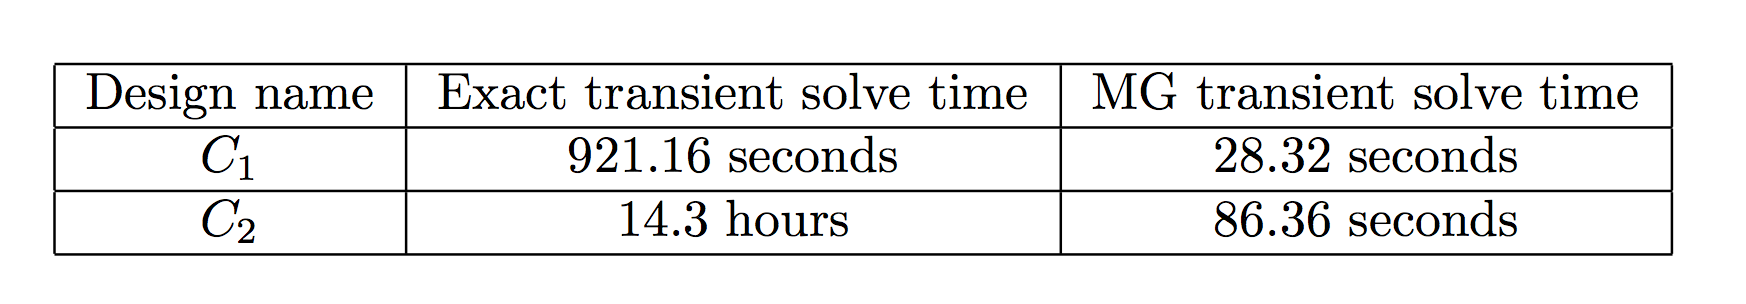
\includegraphics[height=2cm]{t3}
  \caption{瞬态分析中的网格缩减与运行时间}
  \label{fig:t3}
\end{figure}

最后,仍然要验证瞬态分析中所得到的近似解的准确性。 图\ref{fig:a14}和\ref{fig:a15}分别表示出了设计C1和C2的供电网格的某些节点处的电压波形。 很明显,多重网格技术可以准确地跟踪给定节点处的精确电压波形。 图\ref{fig:a16}和\ref{fig:a17}表示出了电压降中的估计误差(电压降与电压值不同),显示出约16%的最差情况误差。 因此,多网格技术为直流DC以及供电网格的瞬态分析提供了精度相对较高的解,并且具有比常规分析技术显着加速的优点。

\begin{figure}[H] % use float package if you want it here
  \centering
  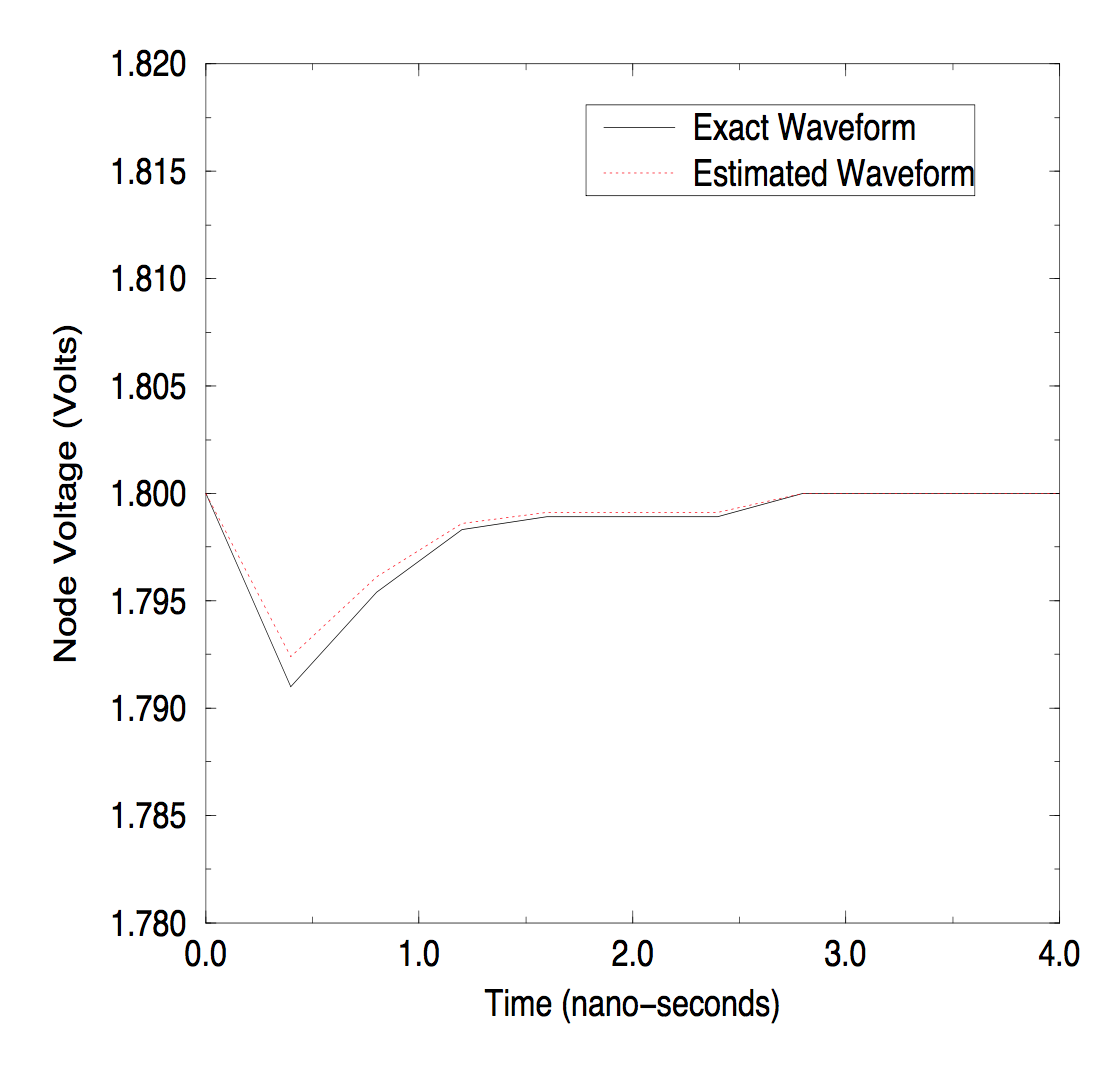
\includegraphics[height=9cm]{a14}
  \caption{C1设计中一个网格节点的电压波形的误差}
  \label{fig:a14}
\end{figure}

\begin{figure}[H] % use float package if you want it here
  \centering
  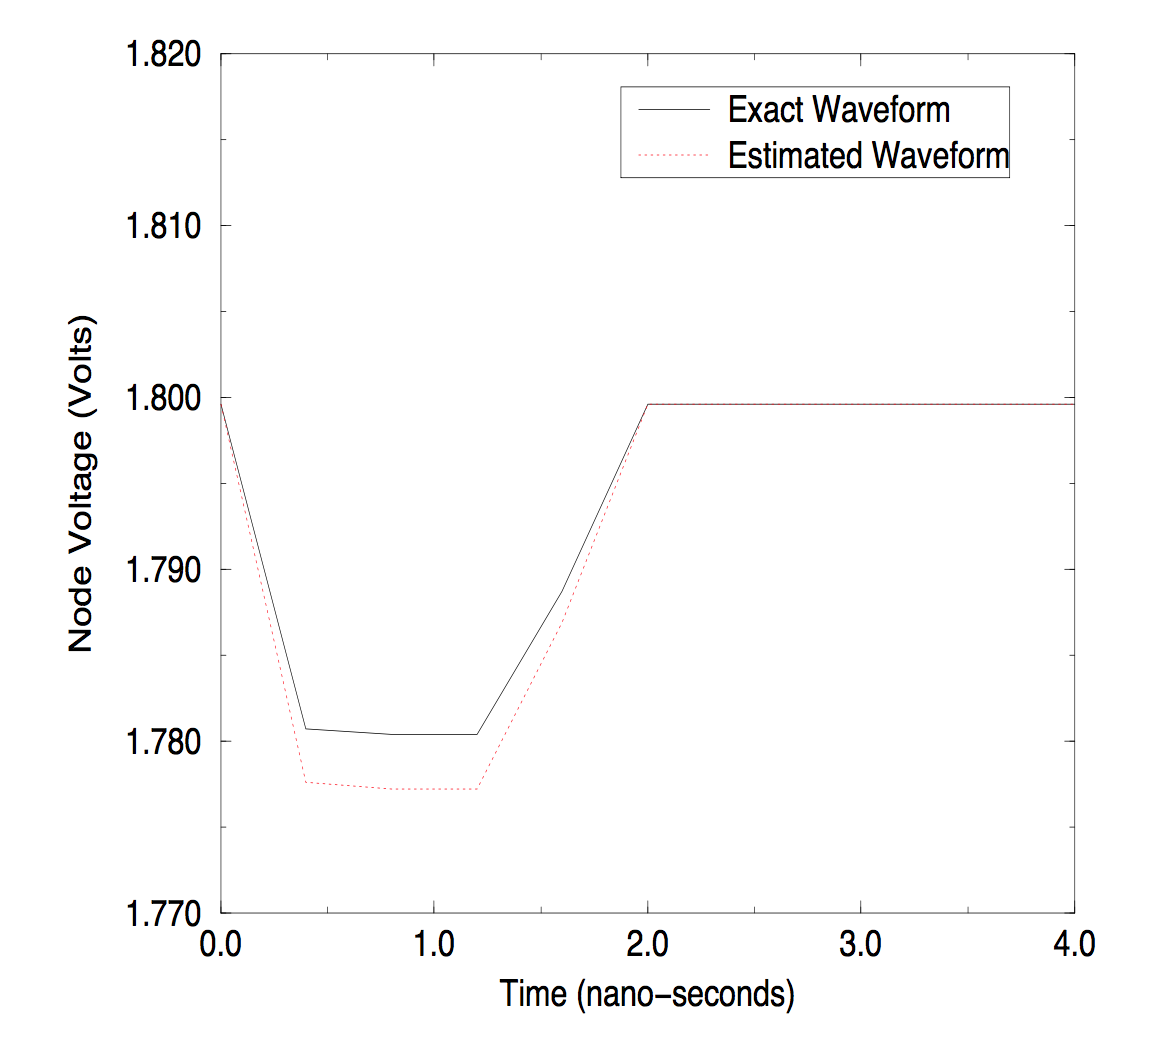
\includegraphics[height=9cm]{a15}
  \caption{C2设计中一个网格节点的电压波形的误差}
  \label{fig:a15}
\end{figure}

\begin{figure}[H] % use float package if you want it here
  \centering
  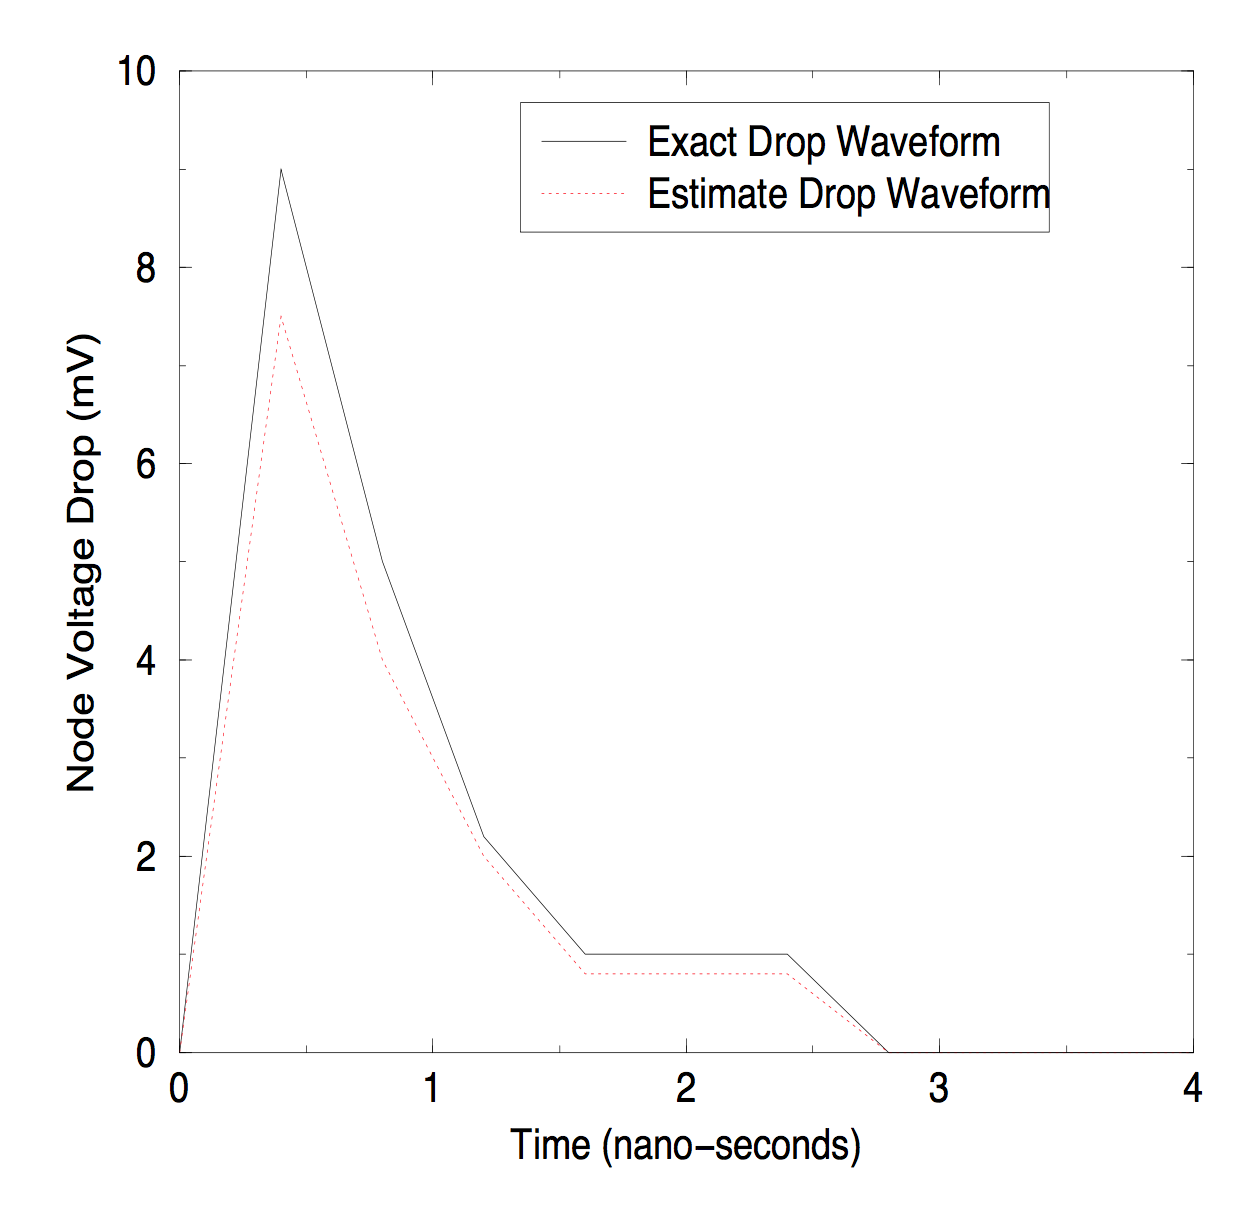
\includegraphics[height=9cm]{a16}
  \caption{C1设计中一个网格节点的电压降波形的误差}
  \label{fig:a16}
\end{figure}

\begin{figure}[H] % use float package if you want it here
  \centering
  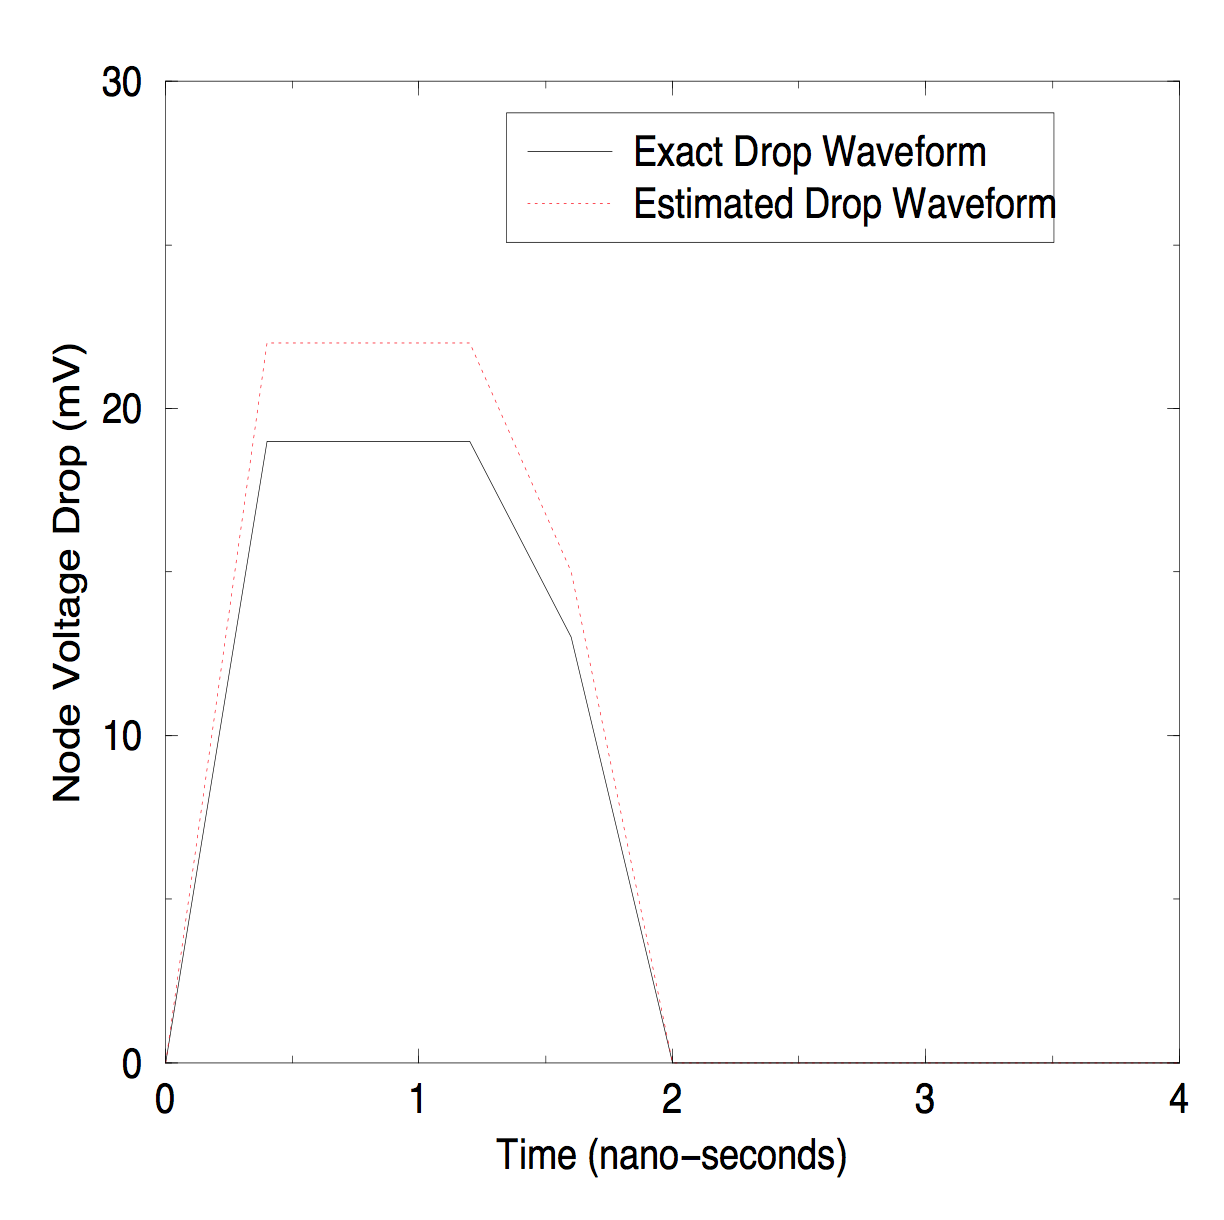
\includegraphics[height=9cm]{a17}
  \caption{C2设计中一个网格节点的电压降波形的误差}
  \label{fig:a17}
\end{figure}


\section{结论}
本文介绍了一种用于供电网格分析的类似于PDE方法的算法。 它遵循广泛用于解决光滑PDE问题的多重网格技术的基本思路。 然而,我们所提出的技术属于直接求解器的类别,因此与常规多重网格方法有着明显的不同,该方法属于迭代求解器类别。 在真实设计上的实验结果表明,使用本文方法的直流和瞬态分析都加速了一到二个数量级。

\section*{参考文献}

\begin{enumerate}[{[}1{]}]
\item Dharchoudhury, Abhijit, et al. "Design and analysis of power distribution networks in PowerPC microprocessors." Proceedings of the 35th annual Design Automation Conference. ACM, 1998.
\item Yim, Joon-Seo, Seong-Ok Bae, and Chong-Min Kyung. "A floorplan-based planning methodology for power and clock distribution in ASICs [CMOS technology]." Design Automation Conference, 1999. Proceedings. 36th. IEEE, 1999.
\item Steele, Gregory, et al. "Full-chip verification methods for DSM power distribution systems." Proceedings of the 35th annual Design Automation Conference. ACM, 1998.
\item Nassif, Sani R., and Joseph N. Kozhaya. "Fast power grid simulation." Proceedings of the 37th Annual Design Automation Conference. ACM, 2000.
\item Zhao, Min, et al. "Hierarchical analysis of power distribution networks." IEEE Transactions on Computer-Aided Design of Integrated Circuits and Systems 21.2 (2002): 159-168.
\item Chen, Howard H., and J. Scott Neely. "Interconnect and circuit modeling techniques for full-chip power supply noise analysis." IEEE Transactions on Components, Packaging, and Manufacturing Technology: Part B 21.3 (1998): 209-215.
\item Pillage, Lawrence. Electronic Circuit \& System Simulation Methods (SRE). McGraw-Hill, Inc., 1998.
\item Nagel, Laurence W. "SPICE2: A computer program to simulate semiconductor circuits." ERL Memo ERL-M520 (1975).
\item Golub, Gene H., and Charles F. Van Loan. Matrix computations. Vol. 3. JHU Press, 2012.
\item Berman, Abraham, and Robert J. Plemmons. Nonnegative matrices in the mathematical sciences. Society for Industrial and Applied Mathematics, 1994.
\item Briggs, William L., Van Emden Henson, and Steve F. McCormick. A multigrid tutorial. Society for Industrial and Applied Mathematics, 2000.
\item Brandt, Achi. "Multi-level adaptive technique (MLAT) for fast numerical solution to boundary value problems." Proceedings of the Third International Conference on Numerical Methods in Fluid Mechanics. Springer Berlin/Heidelberg, 1973.
\item Hackbusch, Wolfgang. Multi-grid methods and applications. Vol. 4. Springer Science \& Business Media, 2013.
\item Brandt, Achi. "Multi-level adaptive technique (MLAT) for fast numerical solution to boundary value problems." Proceedings of the Third International Conference on Numerical Methods in Fluid Mechanics. Springer Berlin/Heidelberg, 1973.
\item Stüben, Klaus, and Ulrich Trottenberg. "Multigrid methods: Fundamental algorithms, model problem analysis and applications." Multigrid methods. Springer Berlin Heidelberg, 1982. 1-176.
\item Ruge, John W., and Klaus Stüben. "Algebraic multigrid." Multigrid methods 3.13 (1987): 73-130.
\end{enumerate}

\chapter{数据集样例数据}

第四节中的Spice格式样例数据如下:
\begin{lstlisting}
rr0 n3_0_0 _X_n3_0_0 0.5
v1 _X_n3_0_0 0 1
rr2 n2_125_125 _X_n2_125_125 0.5
v3 _X_n2_125_125 0 0
* layer: M1,VDD net: 1
R4 n1_0_0 n1_50_0 1.25
R5 n1_50_0 n1_100_0 1.25
R6 n1_100_0 n1_150_0 1.25
R7 n1_0_50 n1_50_50 1.25
R8 n1_50_50 n1_100_50 1.25
R9 n1_100_50 n1_150_50 1.25
R10 n1_0_100 n1_50_100 1.25
R11 n1_50_100 n1_100_100 1.25
R12 n1_100_100 n1_150_100 1.25
R13 n1_0_150 n1_50_150 1.25
R14 n1_50_150 n1_100_150 1.25
R15 n1_100_150 n1_150_150 1.25
* vias from: 1 to 3
V16 n1_0_0 n3_0_0 0.0
V17 n1_0_50 n3_0_50 0.0
V18 n1_0_100 n3_0_100 0.0
V19 n1_0_150 n3_0_150 0.0
V20 n1_50_0 n3_50_0 0.0
V21 n1_50_50 n3_50_50 0.0
V22 n1_50_100 n3_50_100 0.0
V23 n1_50_150 n3_50_150 0.0
V24 n1_100_0 n3_100_0 0.0
V25 n1_100_50 n3_100_50 0.0
V26 n1_100_100 n3_100_100 0.0
V27 n1_100_150 n3_100_150 0.0
V28 n1_150_0 n3_150_0 0.0
V29 n1_150_50 n3_150_50 0.0
V30 n1_150_100 n3_150_100 0.0
V31 n1_150_150 n3_150_150 0.0
* layer: M2,VDD net: 3
R32 n3_0_0 n3_0_50 1.25
R33 n3_0_50 n3_0_100 1.25
R34 n3_0_100 n3_0_150 1.25
R35 n3_50_0 n3_50_50 1.25
R36 n3_50_50 n3_50_100 1.25
R37 n3_50_100 n3_50_150 1.25
R38 n3_100_0 n3_100_50 1.25
R39 n3_100_50 n3_100_100 1.25
R40 n3_100_100 n3_100_150 1.25
R41 n3_150_0 n3_150_50 1.25
R42 n3_150_50 n3_150_100 1.25
R43 n3_150_100 n3_150_150 1.25
* layer: M1,GND net: 0
R44 n0_25_25 n0_75_25 1.25
R45 n0_75_25 n0_125_25 1.25
R46 n0_25_75 n0_75_75 1.25
R47 n0_75_75 n0_125_75 1.25
R48 n0_25_125 n0_75_125 1.25
R49 n0_75_125 n0_125_125 1.25
* layer: M2,GND net: 2
R50 n2_25_25 n2_25_75 1.25
R51 n2_25_75 n2_25_125 1.25
R52 n2_75_25 n2_75_75 1.25
R53 n2_75_75 n2_75_125 1.25
R54 n2_125_25 n2_125_75 1.25
R55 n2_125_75 n2_125_125 1.25
* vias from: 0 to 2
V56 n0_25_25 n2_25_25 0.0
V57 n0_25_75 n2_25_75 0.0
V58 n0_25_125 n2_25_125 0.0
V59 n0_75_25 n2_75_25 0.0
V60 n0_75_75 n2_75_75 0.0
V61 n0_75_125 n2_75_125 0.0
V62 n0_125_25 n2_125_25 0.0
V63 n0_125_75 n2_125_75 0.0
V64 n0_125_125 n2_125_125 0.0
*
iB0_0_v n1_0_0 0 0.3125m
iB0_0_g 0 n0_25_25 0.3125m
iB0_1_v n1_0_50 0 0.3125m
iB0_1_g 0 n0_25_25 0.3125m
iB0_2_v n1_0_100 0 0.3125m
iB0_2_g 0 n0_25_75 0.3125m
iB0_3_v n1_0_150 0 0.3125m
iB0_3_g 0 n0_25_125 0.3125m
iB0_4_v n1_50_0 0 0.3125m
iB0_4_g 0 n0_25_25 0.3125m
iB0_5_v n1_100_0 0 0.3125m
iB0_5_g 0 n0_75_25 0.3125m
iB0_6_v n1_50_50 0 0.3125m
iB0_6_g 0 n0_25_25 0.3125m
iB0_7_v n1_50_100 0 0.3125m
iB0_7_g 0 n0_25_75 0.3125m
iB0_8_v n1_100_50 0 0.3125m
iB0_8_g 0 n0_75_25 0.3125m
iB0_9_v n1_100_100 0 0.3125m
iB0_9_g 0 n0_75_75 0.3125m
iB0_10_v n1_50_150 0 0.3125m
iB0_10_g 0 n0_25_125 0.3125m
iB0_11_v n1_100_150 0 0.3125m
iB0_11_g 0 n0_75_125 0.3125m
iB0_12_v n1_150_0 0 0.3125m
iB0_12_g 0 n0_125_25 0.3125m
iB0_13_v n1_150_50 0 0.3125m
iB0_13_g 0 n0_125_25 0.3125m
iB0_14_v n1_150_100 0 0.3125m
iB0_14_g 0 n0_125_75 0.3125m
iB0_15_v n1_150_150 0 0.3125m
iB0_15_g 0 n0_125_125 0.3125m
\end{lstlisting}

\end{appendix}

%% 本科生进行格式审查是需要下面这个表格,答辩可能不需要。选择性留下。
% 综合论文训练记录表
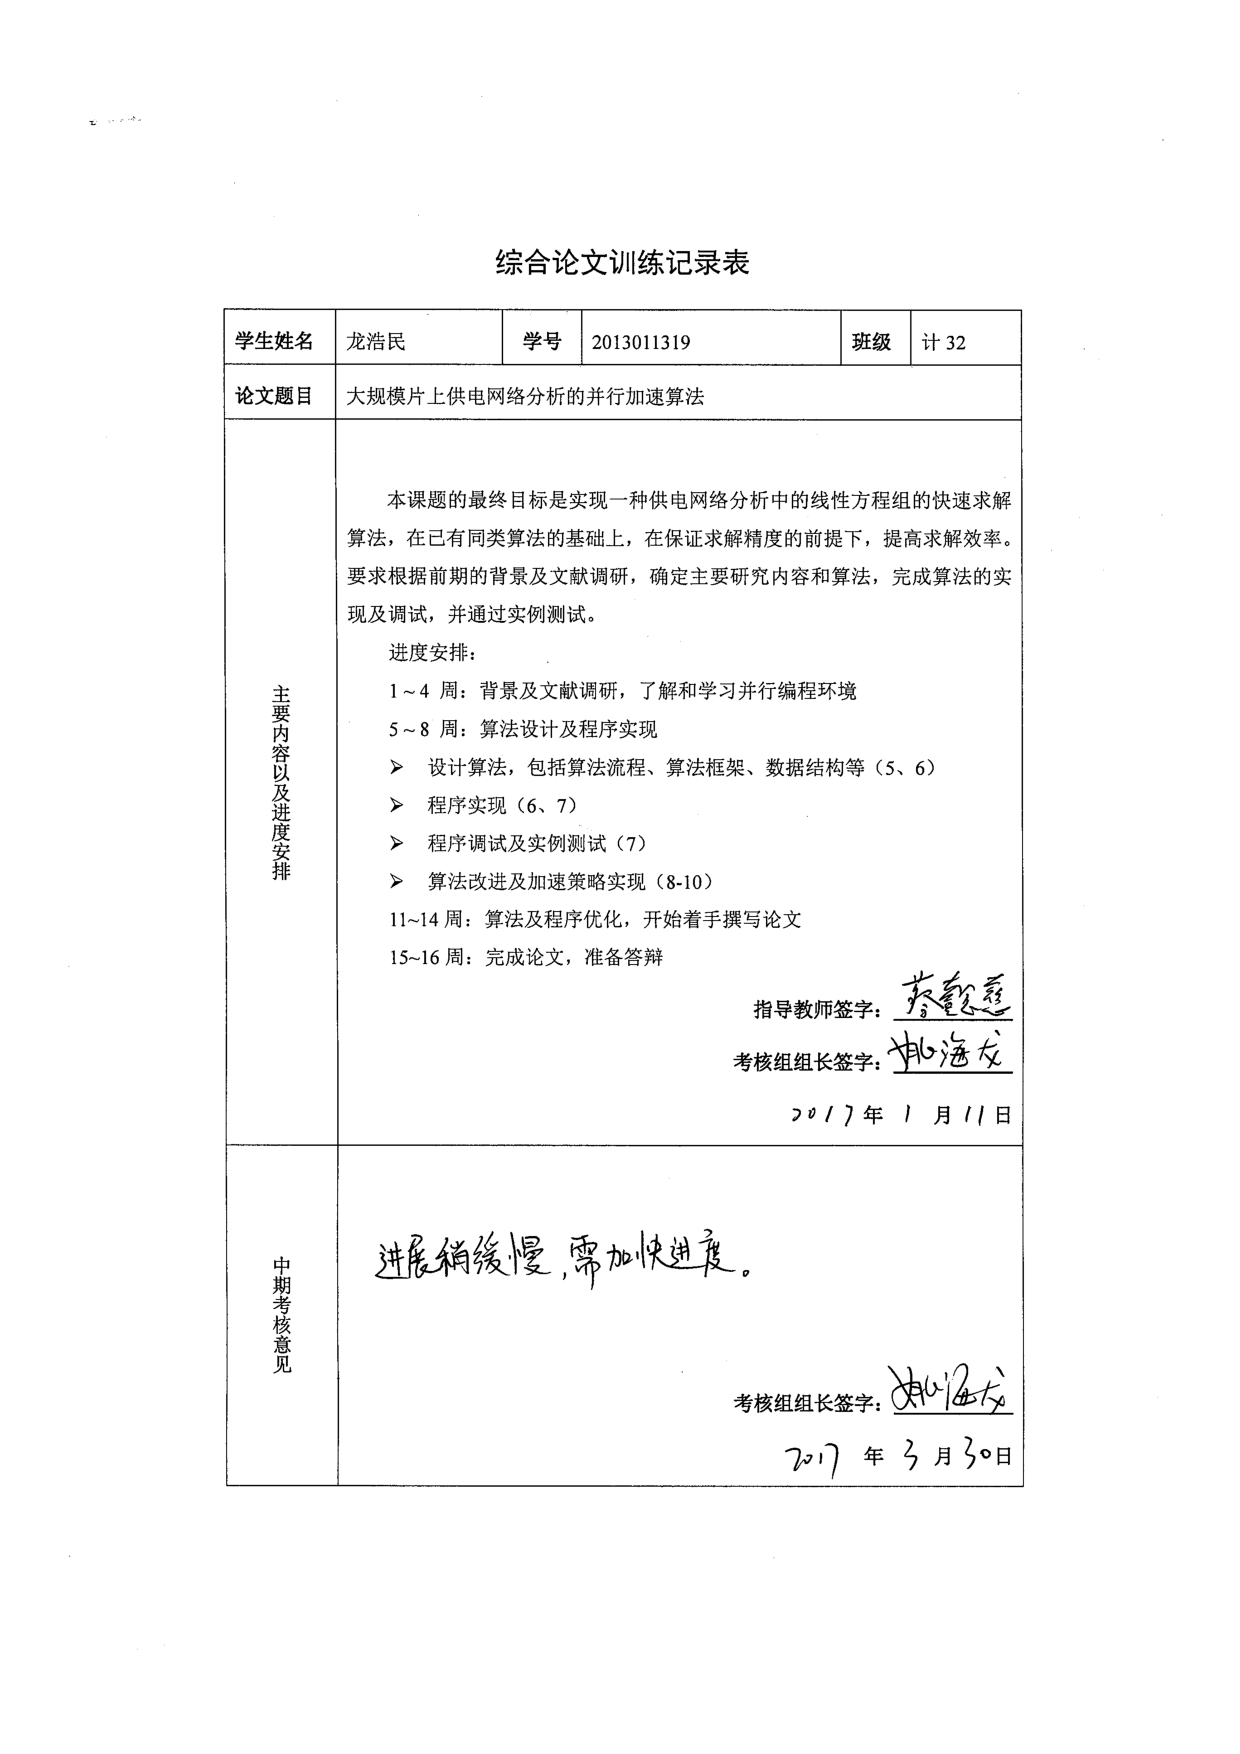
\includepdf[pages=-]{scan-record.pdf}
\end{document}
